\kap{Scattering Theory}\label{chap:scattering}
%\begin{flushleft}

In this chapter much of the theoretical theory for the Nucleon-Nucleon (NN) scattering is derived, 
focusing on deriving practical expressions later used in the computer program. i.e. 
formulas for The S-matrix, T-matrix, phase shifts and inelasticities.
Instead of working with the exact quantum field theory, we develop an approximation from it that involves a S-matrix.
This S-matrix is analog to the familiar S-matrix in classical scattering theory.
So much of the space will be dedicated to deriving central formulas in scattering theory.
And how one derive different S-matrixes from quantum field theory.
One also have to introduce a special S matrix for coupled channels. Deuteron is a bound state of a
proton and a neutron, 
and is an example of such a case. To deal with coupled channels, one have to 
define a mixing parameter along with the phase shift.

Later will also simple potential models be derived. Potentials like the box potential and the parameterized
potential are primitive, but they give a good physical understanding of the NN interactions. The box potential
is also a good way of testing the computational methods that calculate the phase shift, 
since its theoretical phase shift is easy to calculate.
%\nl
%\nl



%Many of the equations I have used in in the computer programs are taken 
%directly from non relativistic scattering theory based on quantum mechanics.
%Therefor I feel it is natural to first derive the equations I use. Mainly focusing on 
%finding practical expressions for The S-matrix, T-matrix, phase shifts and inelasticities.
%\nl
%\nl
\section{Perturbation Theory} 

A Nucleon-Nucleon or a general multiple nucleon system is described by a Hamiltonian 
$\op{H}$ which can be divided into two parts
$\op{H}=\op{H_0}+\op{V}$. Where the dominant part is the unperturbation Hamiltonian $\op{H_0}$ whitch
contains information of each nucleon in absence of the others, and $\op{V}$ is this
interaction term between the nucleons. The time independent {\SE} can be written as
%                                                 
\begin{equation}\label{eq:timeindependentSL}
\big( \op{H_0} +\op{V} \big)\ket{\psi_{\bf k}} = E_{\bf k} \ket{\psi_{\bf k}} 
\end{equation}
%                                                 
$\ket{\psi_{\bf k}}$ can be divided into two orthogonal parts
$\ket{\psi_{\bf k}}=\ket{\phi_{\bf k}}+\ket{\chi_{\bf k}}$ . Where $\ket{\phi_{\bf k}}=\ket{{\bf k}}$
is the free part, and $\ket{\chi_{\bf k}}$ is the perturbated part.
So we have the unperturbated equation
we are familiar with
%                                                 
\begin{equation}
\op{H_0}\ket{\phi_{\bf k}}=\frac{\op{{\bf k}}^2}{2m}\ket{\phi_{\bf k}}=E_{\bf k}\ket{\phi_{\bf k}}
\end{equation} 
%                                                 
Now using the free Greens function defined as
%                                                 
\begin{equation}\label{eq:fgreen}
\op{G}^{(\pm)}_0(E)=\lim_{\epsilon \rightarrow 0} \inv{E-\op{H}_0\pm i\epsilon}
\end{equation}
%                                                 
Where $\epsilon$ is a regulator that decides if the green operator is carrying the state
forward or backwards in time.
We can now rewrite $\ket{\psi_{\bf k}}$ as an iteration equation
 %                                                 
\begin{equation}\label{eq:ket}
\ket{\psi_{\bf k}^{\pm}}=\ket{\phi_{\bf k}}+\op{G}^{(\pm)}_0(E_{\bf k})\;\op{V}\;\ket{\psi_{\bf k}^{\pm}}
\end{equation}
%                                                 
It's easy to verify that state satisfies the time independent \SE 
%                                                 
\begin{equation}
(E-\op{H}_0)\;\ket{\psi_{\bf k}^{\pm}}=\op{V}\ket{\psi_{\bf k}^{\pm}}
\end{equation} 
%                                                 
we have
%                                                 
\begin{equation} 
(E-\op{H}_0)\;\ket{\phi_{\bf k}}=0
\end{equation}
%                                                 
and
%                                                 
\begin{equation}
(E-\op{H}_0)\;\op{G}^{(\pm)}_0(E_{\bf k})\;\op{V}\;\ket{\psi_{\bf k}^{\pm}}=\op{V}
\end{equation}
%                                                 
%                                                 
So (~\ref{eq:ket}) is therefor exact.  
We use the expression "Born approximation of order n" to say how many
times we iterate this equation and where we end the last iteration with the approximation
$\ket{\psi_{\bf k}}=\ket{\bf k}$ Using that $\ket{\phi_{\bf k}}=\ket{\bf k}$
and iterate infinite times we will get
%                                                 
\begin{equation}\label{eq:G}
\ket{\psi_{\bf k}^{\pm}}=\big(1+\op{G}^{(\pm)}(E_{\bf k})\;\op{V}\big)\;\ket{\bf k}
\end{equation}
%                                                 
where
%                                                 
\begin{eqnarray}\label{eq:GG}
\op{G}^{(\pm)} &=& \op{G}^{(\pm)}_{0}+\op{G}^{(\pm)}_{0}\op{V}\op{G}^{(\pm)} \nonumber\\
&=&
\op{G}^{(\pm)}_{0}+\op{G}^{(\pm)}_{0}\op{V}\op{G}^{(\pm)}_{0}
+\op{G}^{(\pm)}_{0}\op{V}\op{G}^{(\pm)}_{0}\op{V}\op{G}^{(\pm)}_{0}+\ldots
\end{eqnarray}
%                                                 
If we now make use of the general operator relation
%                                                 
\begin{equation}
\inv{\op{A}+\op{B}}=\inv{\op{A}}+\inv{\op{A}}\op{B}\inv{\op{A}}+\inv{\op{A}}\op{B}
\inv{\op{A}}\op{B}\inv{\op{A}}+\ldots
\end{equation}
%                                                 
We see that
%                                                 
\begin{equation}
\op{G}^{(\pm)}(E)=\inv{E-\op{H}_0-\op{V}\pm i\epsilon}
\end{equation}
%                                                 
Now $\op{G}^{(\pm)}(E)$ is the Green function for the full Hamilton operator 
$\op{H}=\op{H_0}+\op{V}$ and we can write the time independent {\SE} 
(~\ref{eq:timeindependentSL}) as
%                                                 
\begin{equation}
\big(E_{\bf k}-\op{H}\big)\ket{\psi_{\bf k}^{\pm}}=0
\end{equation}
%                                                 
Where an expression of $\ket{\psi_{\bf k}^{\pm}}$ is given in (~\ref{eq:G})






\section{S- and T-matrix}
%putt inn en figur se vinkel nedenfor!!!!!!!!!!!!!!!!!!!!!!!!!!!!!!!!!!!!!!
%se Hemmer s 262




The scattering operator or also often called the  S-matrix is defined by
%                                                 
\begin{equation}
S({\bf{p}},{\bf{k}})=\braketm{\bf{p}}{\op{S}}{\bf{k}}=\braket{\psi_{\bf{p}}^{-}}{\psi_{\bf{k}}^{+}} 
\end{equation}
%                                                 
This definition tells us that $S(\op{p},\op{k})$ must be the probability
amplitude of finding a free incoming particle in state $\ket{\op{k}}$ which is an 
eigenstate of the free Hamiltonian and a free outgoing particle in state $\ket{\op{p}}$.
And $\op{p}$ is in the direction of the scattering angle $\theta$. Where $\theta$ 
is the angle between $\op{p}$ and $\op{k}$. Since $\op{V}$ 
and$\op{H}_0$ are operators of observables they must be Hermitian. That is $\op{V}=\op{V}^\dagger$ and
$\op{H}_{0}=\op{H}^{\dagger}_{0}$. From this follows
%                                                 
\begin{equation}
(\op{G}^{(\pm)})^\dagger=\op{G}^{(\mp)}
\end{equation}
%                                                 
We  see that  by taking the Hermitian adjunct on both sides of $(~\ref{eq:G})$ 
we get
%                                                 
\begin{equation}\label{eq:Gdagger}
\bra{\psi_{\bf k}^{\pm}}=\bra{\op k}\big(1+\op{V}\;\op{G}^{(\mp)}(E_{\bf k})\big)
\end{equation}
%                                                 
From definition should $\braket{\psi_{\bf{p}}^{+}}{\psi_{\bf{k}}^{+}}$ have
the same probability amplitude as $\braket{\bf{p}}{\bf{k}}$. That is
%                                                 
\begin{equation}
\braket{\psi_{\bf{p}}^{+}}{\psi_{\bf{k}}^{+}}=\braket{\bf{p}}{\bf{k}}
\end{equation}
%                                                 
We now use a little trick where we add zero. 
%                                                 
\begin{eqnarray}
\braket{\psi_{\bf{p}}^{-}}{\psi_{\bf{k}}^{+}} &=&
\braket{\psi_{\bf{p}}^{+}}{\psi_{\bf{k}}^{+}}+\big(\bra{\psi_{\bf{p}}^{-}}
-\bra{\psi_{\bf{p}}^{+}}\big)\ket{\psi_{\bf{k}}^{+}}\nonumber\\
&=&
\braket{{\bf{p}}}{{\bf{k}}}+\bigg( \inv{E_{\bf{p}}-E_{\bf{k}}+i\epsilon}-
\inv{E_{\bf{p}}-E_{\bf{k}}-i\epsilon}\bigg) \braketm{\bf{p}}{\op{V}}{\psi_{{\bf k}}^{+}}
\end{eqnarray}
%                                                 
If we use the relations
%                                                 
\begin{eqnarray}\label{eq:P1}
\inv{x+i\epsilon}={\cal P} \inv{x}-i\pi\delta (x)\\\label{eq:P2} 
\inv{x-i\epsilon}={\cal P} \inv{x}+i\pi\delta (x)
\end{eqnarray} 
%                                                 
Where ${\cal P}$ is Cauchy's principal value. Using these equations we have a well-known expression for the S-matrix
%                                                 
\begin{equation}\label{eq:Sgenerel} 
S({\bf{p}},{\bf{k}})=
\braket{\psi_{\bf{p}}^{(-)}}{\psi_{\bf{k}}^{(+)}}=\braket{{\bf{p}}}{{\bf{k}}}
-2\pi i \delta (E_{\bf p}-E_{\bf k})
\braketm{{\bf p}}{\op{T}}{\bf{k}}
\end{equation}
%                                                 
Or on a more abstract form the S operator can be written as:
%                                                 
\begin{equation}\label{eq:Smat} 
\op{S}=\op{1}-2\pi i \delta (\op{H}_0-E){\op{T}}
\end{equation}
%                                                 
Where we have introduced the transition operator $\op{T}$ which is defined
%                                                 
\begin{equation}\label{eq:Tdef}
\op{V}\ket{\psi_{\bf k}^{(+)}}=\op{T}\ket{{\bf k}}
\end{equation}
%                                                 
From (\ref{eq:ket}) and (\ref{eq:GG}) we see that $\op{T}$ also can be written as:
%                                                 
\begin{equation}\label{eq:TM} 
\op{T}=\op{V}+\op{V}\op{G}^{(+)}\op{V}=\op{V}+\op{V}\op{G}^{(+)}_0\op{T} 
\end{equation}
%                                                 
This is the $\LS$ equation on a general operator form.
A useful feature of the S-matrix when programming is the unitarity of the S-matrix when the potential is real.
Which means that we have elastic scattering.
In such a scattering we must therefore have $SS^{\dagger}=\op{1}$. This is easy to check in the program.
If $SS^{\dagger}\ne \op{1}$ then something is wrong in the program. We can prove this unitarity
by shoving  that $\braketm{{\bf p}}{\op{S}\op{S}^{\dagger}}{{\bf k}}=
\braket{{\bf p}}{{\bf k}}$. We note that
%                                                 
\begin{eqnarray}
\op{S}\ket{{\bf k}}=\ket{{\bf k}}-2\pi i \delta (H_0-E_{\bf k}){\op{T}}\ket{{\bf k}}\\
\bra{{\bf p}}\op{S}^{\dagger}=\bra{{\bf p}}
+\bra{{\bf p}}{\op{T}}^{\dagger}  2\pi i \delta (H_0-E_{\bf p}) 
\end{eqnarray}
%                                                 
Putting these two equations together we have
%                                                 
\begin{eqnarray}\label{eq:Uni} 
\braketm{{\bf p}}{\op{S}^{\dagger}\op{S}}{{\bf k}} &=&
\braket{{\bf p}}{{\bf k}}-2\pi i \delta (E_{\bf k}-E_{\bf p})\braketm{{\bf p}}
{(\op{T}-\op{T}^{\dagger})}{{\bf k}}\nonumber\\
& &
-(2\pi i)^2 
\braketm{{\bf p}}{\op{T}^{\dagger}\delta (E_{\bf k}-H_0 ) \delta (E_{\bf p}-H_0 )
\op{T}}{{\bf k}}
\end{eqnarray}
%                                                 
So we have to show that term 2 and 3 on the right-hand side of (\ref{eq:Uni}) cancel 
each other. From (\ref{eq:TM}) we have $\op{T}=\op{V}+\op{V}\op{G}^{(+)}_0\op{T}$. 
From this we get the relation
%                                                 
\begin{equation}\label{eq:TMC} 
\op{T}^{\dagger}=\op{V}+\op{T}^{\dagger}\op{G}^{(-)}_0\op{V}
\end{equation}
%                                                 
If we use (\ref{eq:TM}) in (\ref{eq:TMC})  we get
%                                                 
\begin{equation}\label{eq:TMCT}
\op{T}^{\dagger}=\op{V}+\op{T}^{\dagger}\op{G}^{(-)}_0\op{T}-\op{T}^{\dagger}
\op{G}^{(-)}_0\op{V}\op{G}^{(+)}_0\op{T}
\end{equation}
%
Do the same with (\ref{eq:TM}). That is, substitute the last $V$ in (\ref{eq:TM}) with
%
\begin{equation}
\op{V}=\op{T}^{\dagger}-\op{V}\op{G}^{(+)}_0\op{T}
\end{equation}
%
and
%
\begin{eqnarray}\label{eq:bevisT}
\op{T}^{\dagger}-\op{T} &=& \op{V}+\op{T}^{\dagger}\op{G}^{(-)}_0\op{T}-\op{T}^{\dagger}
\op{G}^{(-)}_0\op{V}\op{G}^{(+)}_0\op{T}\nonumber\\
& &
-\big[\op{V}+\op{T}^{\dagger}\op{G}^{(+)}_0\op{T}-\op{T}^{\dagger}
\op{G}^{(-)}_0\op{V}\op{G}^{(+)}_0\op{T}\big]\nonumber\\
&=&
\op{T}^{\dagger}\op{G}^{(-)}_0\op{T}-\op{T}^{\dagger}\op{G}^{(+)}_0\op{T}\nonumber\\ 
&=&
\op{T}^{\dagger}\big[\op{G}^{(-)}_0-\op{G}^{(+)}_0\big]\op{T}\nonumber\\
&=&
\op{T}^{\dagger}\bigg[\inv{E-\op{H}_0-i\epsilon}-
\inv{E-\op{H}_0+i\epsilon}\bigg]\op{T}\nonumber\\ 
&=& 
2\pi i \op{T}^{\dagger} \delta (E-\op{H}_0 )\op{T}
\end{eqnarray}
%                                                 
Where $E$ is either $E_{\bf k}$ or $E_{\bf p}$ and we have used (\ref{eq:P1}) and (\ref{eq:P2}) in the last step 
. Noting that
%
\begin{equation}
\delta (E_{\bf k}-H_0 ) \delta (E_{\bf p}-H_0 ) = 
\delta (E_{\bf k}-E_{\bf p} ) \delta (E-H_0 ) 
\end{equation}
%
Finally the 2. and 3. terms on the right-hand side of (\ref{eq:Uni}) will
cancel each other. And therefor the S-matrix must be unitary in this case.
\newline
\newline
In the case of the scattering process we have ($E>0$).

When we want to insert a complete set of
eigenstates in the Green function, we only include the states with positive $E$. i.e.
we remove the bound states from the complete set of eigen states. We are then  
left with the continuous specter of momentum as a basis.
This will be a  projection of (\ref{eq:TM}) into momentum space. 
It's convenient to work in momentum space since 
we then have an integral equation instead of a differential equation when solving it in coordinate space 
(The $\SE$ equation). 
%The interaction potential $V$
%is dependent on the relative 
%distance between the particles. By doing a transformation of $V$ into momentum space, which is
%a Fourier transformation. 
%We have a local potential that is only dependent upon the relative velocities.
If we now use the ket relation found in (\ref{eq:ket}) with the definition of T (\ref{eq:Tdef}), we have 
%
\begin{eqnarray}  
\ket{\psi_{\bf k}^{+}} &=& \ket{{\bf k}}+\op{G}^{(+}_0(E_{\bf k})\;\op{V}\;
\ket{\psi_{\bf k}^{+}} \nonumber\\ 
&=&
\ket{{\bf k}}+ \inv{E_{\bf k}-\op{H}_0+i\epsilon}   \;\op{T}\;
\ket{{\bf k}}\nonumber\\
&=&
\ket{{\bf k}}+ \inv{(2\pi)^3}\int^{\infty}_{\infty}d^3 {\bf q}\quad \ket{{\bf q}}\bra{{\bf q}}
\inv{E_{\bf k}-E_{\bf q}+i\epsilon}   \;\op{T}\;\ket{{\bf k}}
\end{eqnarray}  
%
Where we in the last step inserted a complete set of positive energy states.
By multiplying this equation with $\bra{{\bf p}}\op{V}$ from the left, we get 
%
\begin{equation}\label{eq:Tmatp}
\braketm{{\bf p}} {\op{T}(E)}{{\bf k}} =\braketm{{\bf p}}{\op{V}}{{\bf k}}
+ \inv{(2\pi)^3}\int^{\infty}_{\infty}d^3 { q} \quad\bra{{\bf p}}\op{V}\ket{{\bf q}}\bra{{\bf q}}
\inv{E_{\bf k}-E_{\bf q}+i\epsilon}   \;\op{T}(E)\;\ket{{\bf k}}
\end{equation}
%
Where $E$ is the on-shell energy.

This $\LS$ equation has almost the same form as the one I use in my computer program.
To get the form which 
I use, one has to do a partial wave decomposition of (\ref{eq:Tmatp}). 
This can be practical if the potential is central/local, i.e.        %SJEKK DETTE
$V({\bf r}_1{\bf r}_2)=V({\bf r})$. So that $\Delta\times V({\bf r})=0$.
We are then able to reduce the two particle problem to a one particle problem by
working in the mass center system, where we use the particles relative coordinates ({\bf r}). 
%The transformation from lab- too MC-system of the $\SE$,
%is done later in this chapter.
A local potential has therefor spherical symmetry
with respect to the two particles relative coordinates ${\bf r}$.
This way we have reduced the three-body force to a familiar two-body force.
We can make such a potential by using
meson theory if we assume single wave channel as a good approximation. For example the 
One Boson Exchange model (OBE) is based upon this approximation, which is done by approximating all
higher wave channels by a fictive/effective $\sigma$ meson.

%For a general local potential $V=V(r)$ we can transform it to 
%momentum space by doing a Fourier transform.

We note that $\exp (i{\bf kr})$ can be written in terms of Legendre polynomials 
$P_l({\bf \op{k}\op{r}})$ and spherical Bessel functions $j_l ({ kr})$. Which is known as the 
Bauer series
%%%%%%%%%%%%%%%DEF se side 9 i morten not!!!!!!!!!!!!!!!!!!!!!!!!!!!!!!!!!!!!!!!!!!!!!!!!!!!!!!!!!!!!!!!!!!!!!!!!!!!!!!!!!!!!!!!!!!!!!!!!!!!!!!!!!!!!!!!!!!!
%
\begin{equation}
\exp (i{\bf kr})=\sum^{\infty}_{l=0} (2l+1) i^{l} j_{l}(kr)P_l({\bf \op{k}\op{r}})
\end{equation}

Where the angular momentum quantum number $l$ has been introduced. We then have
for a local potential
%
\begin{flushleft} 
\begin{eqnarray}
&&\langle{{\bf p}}|{\op{V}}\ket{{\bf k}} =\int^{\infty}_{-\infty}d^3r
\exp (-i{\bf pr})V({\bf r})\exp (i{\bf kr})\nonumber\\
&=&
\int^{\infty}_{-\infty}d^3r
\sum^{\infty}_{l'=0} (2l'+1) i^{-l'} j_{l'}(pr)P_{l'}({\bf \op{p}\op{r}}) V({\bf r})
\sum^{\infty}_{l=0} (2l+1) i^{l} j_{l}(kr)P_l({\bf \op{k}\op{r}})\nonumber\\ 
&=&
2\pi\sum^{\infty}_{l,l'=0}(2l'+1)(2l+1) i^{(l-l')}
\int^{\infty}_{0}dr\;r^2 V(r) j_{l'}(pr)j_{l}(kr) \int^{1}_{-1}d({\cos \theta}) 
P_{l'}({\bf \op{p}\op{r}})P_l({\bf \op{k}\op{r}})\nonumber\\
&=&
4\pi\sum^{\infty}_{l=0} (2l+1) P_{l}({\bf \op{p}\op{k}})
\int^{\infty}_{0}dr\;r^2 V(r) j_{l}(pr)j_{l}(kr) 
\end{eqnarray}
\end{flushleft} 
%
Where the z-axis is taken to be in the direction of the incoming particle (${\bf \op{p}}$).
This is done because we expect to see axial symmetry around the z-axis from the scattering. So 
that ${\bf \op{p}\op{k}}$ denote the angle between ${\bf \op{p}}$ and ${\bf \op{k}}$.
In the last step we used the Legendre polynomial relation

\begin{equation}\label{eq:poly}  
 \int^{1}_{-1}d\big({\cos({\bf \op{p}\op{k}})}\big)P_{l'}({\bf \op{p}\op{r}})P_l({\bf \op{k}\op{r}})
 =\frac{2}{2l+1}\;P_{l}({\bf \op{p}\op{k}})\;\delta_{l,l'}
\end{equation}
%
We then define
%
\begin{equation}\label{eq:V_l_def}
V_l({ p},{ k})=\braketm{{ p}}{{\op{V}}_l}{{ k}}=
\int^{\infty}_{0}dr\;r^2 V(r) j_{l}(pr)j_{l}(kr) 
\end{equation}
%
So we have
%
\begin{equation}
V({\bf p},{\bf k})=
4\pi\sum^{\infty}_{l=0} (2l+1) P_{l}({\bf \op{p}\op{k}}) V_l({ p},{ k})
\end{equation}
%
From the definition of $\op{T}$ we have $\op{V}\ket{\psi_{\bf k}^{(+)}}=\op{T}\ket{{\bf k}} $
. We define $\op{T}_l$ so that it satisfies a similar equation
$\op{V}_l\ket{\psi_{ k}^{(+)}}=\op{T}_l\ket{{ k}} $\; , and we have
%
\begin{equation}\label{eq:TsomTm} 
\braketm{{\bf p}}{T}{{\bf k}}=
4\pi\sum^{\infty}_{l=0} (2l+1) P_{l}({\bf \op{p}\op{k}}) \braketm{{ p}}{T}{{ k}}
\end{equation}
%
By using these relations we have
%
\begin{eqnarray} 
&&\inv{(2\pi)^3}\int^{\infty}_{-\infty}d^3 { q} \quad\bra{{\bf p}}\op{V}\ket{{\bf q}}\bra{{\bf q}} 
\inv{E-E_{\bf q}+i\epsilon}   \;\op{T}(E)\;\ket{{\bf k}} 
\nonumber\\  
&=&
\frac{2}{\pi}\sum^{\infty}_{l,l'=0}\int^{\infty}_{-\infty}d^3 { q}
(2l+1)P_l({{\bf p}}{{\bf q}})V_{l}(p,q)
\inv{E-E_{\bf q}+i\epsilon}
(2l'+1) P_{l'}({\bf \op{q}\op{p}})\bra{q}\op{T}_{l'}(E)\ket{{ k}}\nonumber\\
&=&
%\frac{64\pi^3}{(2\pi)^3}
8\sum^{\infty}_{l=0}(2l+1) P_{l}({\bf \op{p}\op{k}})
\int^{\infty}_{0}dq\quad
V_{l}(p,q)\inv{E-E_{\bf q}+i\epsilon}
\bra{q}\op{T}_{l}(E)\;\ket{{ k}}
\end{eqnarray}
%
We have now a  partial wave expression for all the terms in the $\LS$ (\ref{eq:Tmatp}) equation.
%If we now choose to work in the mass center
, and we can rewrite it as
%
%\begin{eqnarray}
%&&\braketm{{\bf p}} {\sum^{\infty}_{l=0} (2l+1) P_{l'}({\bf \op{p}\op{k}})\op{T}_l(E)}{{\bf k}} =
%\sum^{\infty}_{l=0} (2l+1) P_l({\bf \op{p}\op{k}}) \braketm{{\bf p}}{\op{V}_l}{{\bf k}}\nonumber\\
%&&
%+
%\frac{4\pi^2}{(2\pi)^3}\sum^{\infty}_{l,l'=0}\int^{\infty}_{\infty}d {\bf q} 
%(2l+1)P_l({{\bf p}}{{\bf q}})V_{l}(p,q)
%\inv{E-E_{\bf q}+i\epsilon} 
%(2l'+1) P_{l'}({\bf \op{q}\op{p}})\op{T}_{l'}(E)\;\ket{{\bf k}}\nonumber\\ 
%\end{eqnarray}
%By using (\ref{eq:poly}) again we get
%
\begin{equation}\label{eq:Tmy}
\braketm{{ p}} {\op{T}_l(E)}{{ k}} =\braketm{{ p}}{\op{V}_l}{{ k}}
+ \frac{2}{\pi}\int^{\infty}_{0}d { q}\; q^2 \quad\bra{{ p}}\op{V}_l\ket{{ q}}
\inv{2E-2E_{\bf q}+i\epsilon}  \bra{{ q}} \;\op{T}_l(E)\;\ket{{ k}}
\end{equation}
From (\ref{eq:P1}) and (\ref{eq:P2}) we have
\begin{equation}\label{eq:Tmyekstra}
\inv{2E_{\bf k}-2E_{\bf q}\pm i\epsilon}={\cal P}\inv{2E_{\bf k}-2E_{\bf q}}\mp 
i\pi\delta(2E_{\bf k}-2E_{\bf q})={\cal P}\inv{2E_{\bf k}-2E_{\bf q}}\mp 
\frac{i\pi\delta({ k}-{ q})}{2\big|\frac{\partial E_{\bf q}}{\partial { q}}\big|_{{ k}}}
\end{equation}
Where we have in the last step used the general formula for the delta function.
\begin{equation}\label{eq:deltaf} 
\delta (f(x))=\inv{\big|\frac{\partial f(x)}{\partial x}\big|_{x_0}}\delta (x_0)
\end{equation}
%
%The final expression will depend on if we use relativistic energies or not in the propagator. 
%The relativistic form of $\op{T}$ has to be derived from relativistic scattering theory. 
%For relativistic energies $E_{\bf q}=\sqrt{{\bf q}^2+m^2}$ we have
%\begin{equation}\label{eq:Trel}  
%\bigg|\frac{\partial E_{\bf q}}{\partial {\bf q}}\bigg|_{{\bf k}}=\frac{{\bf k}}{\sqrt{{\bf k}^2+m^2}}
%\end{equation} 
%
For $E_{\bf q}=\frac{{ q}^2}{2m}$ we get
%
\begin{equation}\label{eq:Tnrel}
\bigg|\frac{\partial E_{\bf q}}{\partial { q}}\bigg|_{{ k}}=\frac{{ k}}{m}
\end{equation}
%
So the $\LS$ equation can be written as
%
\begin{eqnarray}\label{eq:Tnrelllll} 
\braketm{{ p}} {\op{T}_l(E_{ k})}{{ k}}&=&\braketm{{ p}}{\op{V}_l}{{ k}}
+ \frac{2m}{\pi}\;{\cal P}\int^{\infty}_{0}d { q}\; q^2 \quad\bra{{ p}}\op{V}_l\ket{{ q}}
\;\inv{{ k^2}-{ q^2}}   \;\bra{{ q}}\op{T}_l(E_{ k})\ket{{ k}}\nonumber\\
&&
-i { k}m \;\bra{{ p}}\op{V_l}\ket{{ k}}
   \;\bra{{ k}}\op{T}_l(E_{ k})\;\ket{{ k}}
\end{eqnarray}
%
Now when we have an expression for $\op{T}_l$ we would like to use it to calculate the phase shifts
and the inelasticities, which are the experimental values we can obtain from such a scattering process.
It turns out that they are very close related to the $\op{S}_l$, which will soon be explained.
If we have an elastic scattering, then $\op{S}$ is unitary as proved earlier in this chapter.
We then have
%
\begin{equation}\label{eq:Slun}
\braketm{{\bf p}}{\op{S}^\dagger \op{S}}{{\bf k}}=\int^{\infty}_{-\infty} d^3 { r}\;
\braketm{{\bf p}}{\op{S}^\dagger }{{\bf r}}\braketm{{\bf r}}{\op{S} }{{\bf k}} 
=\braketm{{\bf p}} {\;\op{1}\;}{{\bf k}}=(2\pi)^3\;\delta ({\bf p}-{\bf k})
\end{equation}
%
We also want to rewrite $\braketm{{\bf r}}{\op{S} }{{\bf k}}$ as a partial
wave expansion
%
\begin{eqnarray}\label{eq:Slutledning}  
\braketm{{\bf r}}{\op{S} }{{\bf k}} 
&=&
\int^{\infty}_{-\infty} \frac{d^3 { q}}{(2\pi)^3}\;\braket{{\bf r}}{{\bf q}}
\braketm{{\bf q}}{\op{S} }{{\bf k}}\nonumber\\
&=&
\int^{\infty}_{-\infty} \frac{d^3 { q}}{(2\pi)^3}\; \exp(i{\bf rp})\big(\;
\braket{{\bf q}}{{\bf k}} -2\pi i\; \delta (2E_{\bf q}-2E_{\bf k})\;\braketm{{\bf q}}{\op{T}}{\bf{k}}\;\big)\nonumber\\  
&=&
\exp(i{\bf rk})-\bigg[ i^{l+1}m\int^{\infty}_{0}dq\;q\;\delta (q-k)\nonumber\\
&&\qquad 
\sum^{\infty}_{l,l'=0}j_{l}(kr)(2l+1)(2l'+1)\;\bra{q}\op{T}_{l}\;\ket{{ k}}\;\int^{1}_{-1}d(\cos\theta)\; P_{l'}
({\bf \op{q}\op{k}})P_{l}({\bf \op{q}\op{r}})\bigg] \nonumber\\
&=& 
\sum^{\infty}_{l=0} (2l+1) i^{l} j_{l}(kr)P_l({\bf \op{k}\op{r}})\big[1-2imk\;\bra{k}\op{T}_{l}\;\ket{{ k}} \big]
\end{eqnarray}
%
Where we have used (\ref{eq:deltaf}) and (\ref{eq:Tnrel}) to rewrite $\delta (2E_{\bf q}-2E_{\bf k})$ for 
$E_{\bf k}=\frac{{\bf k}^2}{2m}$. We define ${\op{S} }_l$ to be
%
\begin{equation}\label{eq:Sl} 
\op{S}_{l}\ =1-2imk\;\bra{k}\op{T}_{l}\;\ket{{ k}}
\end{equation}
%
So that
%
\begin{equation}\label{eq:SSl}
\braketm{{\bf r}}{\op{S} }{{\bf k}} =\sum^{\infty}_{l=0} (2l+1) i^{l} j_{l}(kr)P_l({\bf \op{k}\op{r}})\;\op{S}_{l}
\end{equation}
%
Now we can show that also ${\op{S} }_l$ is unitary if we have an elastic scattering. By
using (\ref{eq:Slun}), (\ref{eq:SSl}) and choosing $|\op{S}_{l}|=1$ for all $l$
%
\begin{equation}\label{eq:SSlun}
\int^{\infty}_{-\infty} d^3 { r}\;
\braketm{{\bf p}}{\op{S}^\dagger }{{\bf r}}\braketm{{\bf r}}{\op{S} }{{\bf k}}
=
\int^{\infty}_{-\infty} d^3 { r}\; \exp(i{\bf r(k-p)})=(2\pi)^3\delta ({\bf p}-{\bf k})
\end{equation}
%
We see that $|\op{S}_{l}|=1$ gives the right result.
\nl
For inelastic scattering we have a complex potential which
makes creation of other particles possible. In this process energies are taken from the nucleons, or even excited
to other barions. 
Since this will reduce the velocity of the nucleons, we also get a reduced flux out after the scattering.
So we always have $|\op{S}_{l}|\le 1$ in a scattering process. The creations of other particles have to
follow certain rules such as the nucleon number, total spin, isospin, momentum, energy and charge are 
conserved in the process. These matters will be discussed later since we need quantum field theory to 
explain creations of new particles. 





\section[Phase shifts and Inelasticities]{The Scattering Amplitude, Phase shifts and Inelasticities}  
%figur!!!!!!!!!!!!!!!!!!!!!!!!!!!!!!!!!!!!!!!!!!!!!!!!!!!!!!
%hemmer s 262
%
The scattering process we now look at, is the situation where a particle is scattered from a
local, stationary potential $V({\bf r})$, which is the same situation we have in the mass center system
if two particles are interacting through a local/central potential.
We can use the time independent $\SE$ 
(\ref{eq:timeindependentSL}) to solve the scattering caused by the potential. 
%If we have a local potential, 
Using $E=\frac{k^2}{m}$ we can write the  $\SE$ as
%
\begin{equation}\label{eq:Slfi} 
({\bf \triangledown}^2+k^2 )\psi ({\bf r})= 2m\; V({\bf r})\;\psi ({\bf r})
\end{equation}
%
Where $\psi ({\bf r}) = \braket{{\bf r}}{\psi}$ is the wave function. The behavior of the wave function
will be very complicated near the scattering center. Further away from this center the potential grows weaker, 
and for large $r$ it can be neglected. And we will have free particle solutions from the $\SE$ equation.
Where the incoming particle is a plane wave and the outgoing/scattered particle is a radial wave.
%
\begin{equation}
\psi ({\bf r})=\psi_{in} ({\bf r})+\psi_{out} ({\bf r})\qquad {\text for}\quad r\to\infty
\end{equation}
And
\begin{equation}
\psi_{in} ({\bf r})=\exp (i{\bf kr})
\end{equation}
For an elastic scattering the kinetic energy is conserved, so the scattered wave must have the same 
wave number $k=|{\bf k}|$ as the incoming wave.
\begin{equation}
\psi_{out} ({\bf r})=f(\theta ,\varphi)\frac{\exp (i{ kr})}{r}
\end{equation}
%
$f(\theta ,\varphi)$ describes the distribution in the different directions and is called
the scattering amplitude. 
So for large $r$ we have
%
\begin{equation}\label{eq:spredamp} 
\psi ({\bf r})=\exp (i{\bf kr}) + f(\theta ,\varphi)\frac{\exp (i{ kr})}{r} 
\end{equation}
%
From (\ref{eq:ket}) we have
%
\begin{equation}\label{eq:ledd}
\braket{{\bf r}}{\psi_{\bf k}^{+}}=\braket{{\bf r}}{{\bf k}}+
\int^{\infty}_{-\infty}d^3 {{ r}'}\;\braketm{{\bf r}}{\op{G}^{(+)}_0(E_{\bf k})}{{\bf r}'}\;
{V}({{\bf r}'})\;\braket{{\bf r}'}{\psi_{\bf k}^{+}} 
\end{equation}
%
Where we need to know the Green function with respect to coordinate space. We have
%
\begin{eqnarray}
\braketm{{\bf r}}{\op{G}^{(+)}_0}{{\bf r}'} 
&=&
\int^{\infty}_{-\infty}\frac{d^3 {{ q}}}{(2\pi)^3}\;
\braketm{{\bf r}}{\inv{E-\op{H}_0+ i\epsilon} }{{\bf q}}\;\braket{{\bf q}}{{\bf r}'} \nonumber\\ 
&=&
\frac{4\pi m}{(2\pi)^3}\;\int^{\infty}_{0}dq\;q^2\int^{\pi}_{0}d\theta\; 
\frac{\sin\theta}{{{ k}^2}-{{ q}^2}+ i\epsilon}\;\exp(iq|{\bf r}-{\bf r}'|\cos\theta) \nonumber\\ 
&=& 
\frac{4\pi m}{(2\pi)^3i|{\bf r}-{\bf r}'|}\;\int^{\infty}_{0}dq\;q\;
\frac{1}{{{ k}^2}-{{ q}^2}+ i\epsilon}\;\bigg[\exp(iqr)-\exp(-iq|{\bf r}-{\bf r}'|)\bigg] \nonumber\\
&=&
\frac{4\pi m}{(2\pi)^3i|{\bf r}-{\bf r}'|}\;\int^{\infty}_{-\infty}dq\;q\;
\frac{1}{{{ k}^2}-{{ q}^2}+ i\epsilon}\;\exp(iq|{\bf r}-{\bf r}'|) \nonumber\\
&=&
-\frac{m}{2\pi |{\bf r}-{\bf r}'|}\exp(ik|{\bf r}-{\bf r}'|)
\end{eqnarray}
%
Where we used that the Green function has a simple pole in $q=+\sqrt{2mE}=k$.  
For $r\gg r'$ we have
\begin{equation} 
|{\bf r}-{\bf r}'|= r
\end{equation}  
\begin{equation} 
k|{\bf r}-{\bf r}'|=k\sqrt{r^2-2{\bf r}{{\bf r}'}+{r'}^2}=kr-\frac{{\bf r}
\cdot{{\bf r}'}}{r}+{\cal O}(\frac{1}{r})
\end{equation}  
%
Going back to (\ref{eq:ledd}) we now get
%
\begin{equation}
\braket{{\bf r}}{\psi_{\bf k}^{+}} \simeq\exp (i{\bf kr}) - \frac{\exp (i{ kr})}{r}\;\frac{m}{2\pi}
\int^{\infty}_{-\infty}d^3 {{ r}'}\;\exp \bigg(-ik\frac{{\bf r\cdot r}'}{r}\bigg)
{V}({{\bf r}'})\;\braket{{\bf r}'}{\psi_{\bf k}^{+}}
\end{equation} 
%
Comparing this with (\ref{eq:spredamp}) we see that the scattering amplitude can be written as
%
\begin{equation}\label{eq:fogT}
f(\theta ,\varphi)=-\frac{m}{2\pi}
\int^{\infty}_{-\infty}d^3 {{ r}'}\;\exp \bigg(-ik\frac{{\bf r\cdot r}'}{r}\bigg)
{V}({{\bf r}'})\;\braket{{\bf r}'}{\psi_{\bf k}^{+}}
\end{equation}
%
or
%
\begin{eqnarray}\label{eq:fogT2} 
f(\theta ,\varphi)
&=&
-\frac{m}{2\pi}
\int^{\infty}_{-\infty}\frac{d^3}{(2\pi)^3{ q}}\int^{\infty}_{-\infty}d^3 {{ r}'}\;
\exp \bigg(i{\bf qr}'-ik\frac{{\bf r\cdot r}'}{r}\bigg)
\braketm{{\bf q}}{\op{V}}{\psi_{\bf k}^{+}}\nonumber\\
&=&
-\frac{m}{2\pi}\braketm{k{\bf \op{r}}}{\op{T}}{{\bf k}}
\end{eqnarray}
%
%
%
%
If we have a local potential we can write the wave function as
%
\begin{equation}
\psi ({\bf r},\theta ,\varphi)=\sum^\infty_{l=0}\sum^l_{m=-l}c_{lm}R_l(r)Y_{lm}(\theta ,\varphi) 
\end{equation}
%
Where the $Y_{lm}$ are spherical harmonics,$c_{lm}$ are constants and 
$R_l(r)$ are radial functions satisfying the radial part of the $\SE$ 
%
\begin{equation}
\frac{d^2}{r^2}(rR_l)+\bigg[ k^2-2mV({\bf r})-\frac{l(l+1)}{r^2}\bigg](rR_l)=0
\end{equation}
%
If the z-axis is taken in the direction of the incoming particles, we get axial symmetry when $m=0$. The
spherical harmonics $Y_{lm}(\theta ,\varphi)\propto P_l^{|m|}\cos\theta e^{im\phi}$ can then be written as
Legendre polynomials
$Y_{lm}(\theta)\propto P_l(\cos\theta)$ and the wave function will be
%
\begin{equation}
\psi ({\bf r},\theta)=\sum^\infty_{l=0}C_l R_l(r)P_{l}(\cos\theta )
\end{equation}
%
$C_l$ are constants. So let us find this partial wave expression of $\psi (r)$. Using the $\SE$ equation
given in (\ref{eq:Slfi}) and look at large  $r$ where the potential can be neglected if
$V(r)\propto 1/r^n$, and $n\gg 1$. We have  
%
\begin{equation}
({\bf \triangledown}^2+k^2 )\psi ({\bf r})=0\qquad {\text for}\quad r\to \infty 
\end{equation}
%
This equation has the general solution
%
\begin{equation}
\psi ({\bf r})=c_l e^{\pm i({\bf kr}+\delta_l)}
\end{equation}
%
Two constants are used to generate the general this solution. $\delta_l$ which is known as the phase shift of
the partial wave with angular momentum $l$, and $c_l$ witch is an arbitrary constant. Since this is a scattering 
process, only the outgoing wave has a physical meaning.
Writing the $e^{ i({\bf kr}+\delta_l)}$ in terms of partial waves
%
\begin{equation}
\psi ({\bf r})\bigg|_{r\to \infty}=c_l\sum^\infty_{l=0}(2l+1)\;i^l j_l({ kr}+\delta_l)\; P_l(\cos\theta)
\end{equation}
%
In the asymptotic region where $r\to \infty$ we can write the spherical Bessel function $j_l(kr+\delta_l)$ as
%
\begin{eqnarray}
j_l(kr+\delta_l)\bigg|_{r\to \infty}
&=&
\inv{kr}\sin\big(kr+\frac{\pi}{2}l+\delta_l\big)\nonumber\\
&=& 
\inv{2ikr}\bigg[e^{i(kr+\frac{\pi}{2}l+\delta_l)}-e^{-i(kr+\frac{\pi}{2}l+\delta_l)}\bigg]
\end{eqnarray}
%
If we then subtract the incoming wave from the total wave function
%
\begin{equation}
\psi ({\bf r})\bigg|_{r\to \infty}-e^{i{ kr}}=\sum^\infty_{l=0}\frac{2l+1}{2ikr}i^l 
\bigg[(c_l e^{ i({ kr}+\delta_l)}-1) e^{ i{ kr}}-(c_l e^{ i({ kr}+\delta_l)}-1) e^{-i{ kr}}\bigg]P_{l}(\cos\theta ) 
\end{equation}
%
This equation contains both incoming and outgoing spherical wave terms for large $r$.
By choosing $c_l=e^{ i\delta_l}$ we can remove the incoming spherical wave
%
\begin{equation}
\psi ({\bf r})\bigg|_{r\to \infty}-e^{i{ kr}}=\frac{e^{ i({\bf kr}}}{2ikr}\sum^\infty_{l=0}(2l+1)\;i^l
\big(e^{ i({\bf kr}+2\delta_l)}-1\big)\;P_{l}(\cos\theta )  
\end{equation}
%
From the definition of the scattering amplitude (\ref{eq:spredamp} ) we obtain $f(\theta)$
which is no longer dependent on $\varphi$ because of the symmetry around the z-axis
%
\begin{equation}\label{eq:fpart}
f(\theta)=\inv{2ik}\sum^{\infty}_{l=0} (2l+1)(e^{2i\delta_l}-1) P_{l}(\cos\theta)
\end{equation} 
%
Or alternatively by using $e^{2i\delta_l}-1=2ie^{i\delta_l}\sin\delta_l$
%
\begin{equation}
f(\theta)=\inv{k}\sum^{\infty}_{l=0} (2l+1)e^{i\delta_l}\;\sin\delta_l\; P_{l}(\cos\theta)
\end{equation}
%
This is the partial wave expansion of the scattering amplitude.


Inserting the expression of $\braketm{{ p}}{T}{{ k}}$ we have from  (\ref{eq:TsomTm}) and 
(\ref{eq:fpart}) for $f(\varphi)$ we get $T_l$ as a function of the partial wave phase shifts
%
\begin{equation}\label{eq:TsomTme} 
\braketm{{ p}}{T}{{ k}}=\inv{2mik}\bigg[1-e^{2i\delta_l}\bigg]
\end{equation}
%
Using this $T_l$ in (\ref{eq:Sl}) we get
%
\begin{equation}\label{eq:deltask}
S_l=e^{2i\delta_l}
\end{equation}
%
%If we have an inelastic scattering, 
We want to define $S_l$ for inelastic scattering, 
in such a way that we can still use methods developed for phase shifts in elastic scattering.
%
%
\begin{equation}\label{eq:deltaski}
S_l=\eta_l\; e^{2i\delta_l}
\end{equation}
%
$\eta_l$ is called the inelasticity, and we will always have $\eta_l\le 1$.
From the definitions, both $\eta_l$ and $\delta_l$ are always real. 
We note that $ e^{2i\delta_l}e^{-2i\delta_l}=1$ which is the same properties as 
$S_l$ has in an elastic scattering, and $\delta_l$ can be found the same way as before! 
\nl
The physical meaning of the inelasticity $\eta_l$, can be explained from the elastic process
\begin{equation}\label{eq:probforelastic}
N+N\to N+N
\end{equation}
All the other processes where we have other particles are created in the process,
are inelastic. $|\eta_l|^2$ can therefor be inteprented as the
probability of elastic scattering (\ref{eq:probforelastic}). This definition of
inelasticity does not contain any information about the relation between all the inelastic processes. Like
the probability of one pion or two pion creation in the scattering. These cases are easy to detect experimentally, and
one can build models to calculate the probability of the different processes.  
\nl
Inelasticity is entering the scattering at about 300 MeV in the lab system, where the lightest $\pi$-mesons
can be created. The inelasticity increases with energy, where other mesons and even meson pair can be created.
The "nna13" potential is a potential that includes the processes that arrive in an OBE-model up to 1GeV.
To be able to describe inelasticity, one need to use a complex potential. Also T-matrix equations are necessary, since
the R-matrix only can handle real potentials.








%We can always have some inelasticity from the Bremsstrahlung ($p+p\to p+p+\gamma)$ in the pp scattering.
%This term is small and will diaper when we neglect the electromagnetic force. Larger inelasticity
%are entering the picture for lab energies about 300 MeV. 
%This is due to
%fact that nucleons have enough energy to create the lightest meson (the $\pi$ mesons).
%We have $N+N\to N+N+\pi$.
%At higher
%energies creations of other mesons will also enter the process. 
%At 600 MeV creation of 2 $\pi$ is possible, but at this energy a more important factor to the inelasticity arrives. 
%This is due to the the excitations of one the nucleons into $\triangle$(1232). 
%This has such a big effect on the inelasticity since it doesn't only slow down the speed of the nucleons, which is what the 
%$\pi$-mesons does. $\triangle$ excitation also remove one nucleon in the process.
%%But the biggest contribution to the
%%inelasticity at higher energies is the 2 mesons exchange that can change one of the incoming nucleons. At
%%lab energies around 600 MeV we can get the 2 $\pi$ exchange through the process
%$N+N\to N+\triangle$. Where $\triangle$ has the same barion number and isospin as the nucleon N it replaced. 
%
%There exist four $\triangle$-barions
%and they come from the isospin-$\frac{2}{3}$ barion group. 
%They can be expressed in terms of quarks as $\triangle^-={\textrm{ddd}}(I_3=-3/2)$,\;$\triangle^-=\textrm{udd}(I_3=-1/2)$,
%\;$\triangle^-={\textrm{uud}}(I_3=1/2)$ and $\triangle^{++}={\textrm{uuu}}(I_3=3/2)$. Where $I_3$ denotes the
%particles isospin. 
%%%If we assume that the isospin is a good quantum number. i.e. we neglect the decays done by the
%%electromagnetic and the week force. 
%Since $n$ has $I_3=-1/2$ and $p$ has $I_3=1/2$ and the electrical charge is always conserved, 
%we have that $p+p\to N+\triangle^{++}$ is possible.
%At energies above 1,2 GeV we can get double $\triangle$ excitations ($N+N\to \triangle+\triangle$). 
%This is possible for both isospin 0 and 1 $N+N\to \triangle+\triangle$
%If we want to include the inelasticity caused by one $\triangle$ excitation using a real potential like the "bonn B"-potential
%, we have to include the width of the $\triangle$-barions in the propagator $G(E)$. 
%This width (self-energy) will be a complex component
%of the energy. The real part will be the same as before. Instead of doing this one can also make use of the complex
%potentials already on the marked. Machleidts "nna13"-potential is for example relatively good up to 1 GeV. This potential
%include both one and two virtual $\triangle$ excitations. This self-energy model is 
%equivalent to the Feynman diagrams were mesons are emitted in the process. One can therefor explain the small
%inelasticity, for low energies, by the small self-energy of N.
%\begin{equation}\label{eq:probforelastic}
%N+N\to N+N
%\end{equation}
%This is the elastic process. All the other processes are inelastic. $|\eta_l|^2$ can therefor be inteprented as the 
%probability of elastic scattering (\ref{eq:probforelastic}). This definition of 
%inelasticity does not contain any information about the relation of all the other inelastic processes. Like
%the probability of one pion or two pion creation in the scattering. 














%\kap{Scattering Theory}\label{chap:scattering} 

\section{The Optical Theorem}
In (\ref{eq:bevisT}) we found that
\begin{eqnarray}\label{eq:bevisT2}
2\;{\cal I}m\{\op{T}\}=
\op{T}-\op{T}^{\dagger} =-2\pi \op{T}^{\dagger} \delta (E-\op{H}_0 )\op{T}
\end{eqnarray}
Were we use lab system.  Taking the matrix element of this equation
\begin{eqnarray}\label{eq:bevisT23}
\braketm{p}{\op{T}}{k}-\braketm{k}{\op{T}}{p}^{\dagger} =-
\frac{2 \pi m}{(2\pi)^3}\int^\infty_{-\infty}d^3q \braketm{k}{\op{T}}{q}^{\dagger}
\braketm{q}{\op{T}}{k}\delta (k-q )
\end{eqnarray}
We can therefor rewrite (\ref{eq:bevisT2}) 
\begin{eqnarray}\label{eq:bevisT24}
{\cal I}m\{\braketm{{\bf k}}{\op{T}}{{\bf k}}\}=
-\pi m k |\braketm{{\bf k}}{\op{T}}{{\bf k}}|^2
\end{eqnarray}
or in partial waves, we have
%
\begin{eqnarray}\label{eq:bevisT2467}
{\cal I}m\{\braketm{{ k}}{\op{T}_l}{{ k}}\}=
-2 m k |\braketm{{   k}}{\op{T}_l}{{ k}}|^2
\end{eqnarray}
%
%
Using the relation between scattering amplitude $f$ and the T-operator $T$ given in
(\ref{eq:fogT2}),
we have the total cross section $\sigma$ for the special case of forward scattering:
\begin{eqnarray}\label{eq:bevisT2hei}
\sigma=\int d\Omega|f(\theta)|^2=\frac{4\pi}{k}{\cal I}m\{ f(0)\}
\end{eqnarray}
%
This is known as the optical theorem, and it relates the scattering cross section 
to the imaginary part of the scattering amplitude in the forward direction of the lab system.

Since we mostly work in the mass center system, we note that (\ref{eq:bevisT2}) 
with a center of mass delta function
$\delta (2E_k-2E_q)$, will give us
\begin{eqnarray}\label{eq:bevisT246}
{\cal I}m\{\braketm{{ k}}{\op{T}_l}{{ k}}\}=
- m k |\braketm{{   k}}{\op{T}_l}{{ k}}|^2
\end{eqnarray}

















\section[Minimal Relativity]{Relativistic Approach Leading to Blankenbecler-Sugar Equation and Minimal Relativity }

%In this section we choose to work in the mass center.
The total relativistic energy in the mass center is $2E_q=2\sqrt{q^2+m^2}$. Inserting relativistic energy in the Green operator
\begin{equation}\label{eq:Grelativisjada}
{\op{G}^\pm_0(E_k)}=\frac{1}{{2E_k}^2+2{\op{H}'}\pm i\epsilon}=\frac{1}{2\sqrt{k^2+m^2}+2\op{H}'\pm i \epsilon}
\end{equation}
%
Where $\op{H}'\ket{{\bf k}}=\sqrt{k^2+m^2}\ket{{\bf k}}$. This propagator
will cause trouble if we want to do a Fourier transformation to coordinate space. 
If we had been able to to this transformation we could have found the exact value of the potential in both systems. 
Which is of big interest. Since we had this property in the non relativistic case, we are tempted to approximate the 
Green operator to the non relativistic case ($\op{H}\ket{{\bf k}}=\frac{k^2}{2m}\ket{{\bf k}}$)
\begin{equation}\label{eq:Gikkerelativis} 
{\op{G}^\pm_0(E_k)}=\frac{m}{{k}^2+2{\op{H}}\pm i\epsilon}
\end{equation}
%
%And use relativistic energies everywhere else.
%
The relativistic on shell scattering amplitude can be written as
\begin{equation}
f_{rel}(\theta)=\frac{{E_p}}{m}f_{class}(\theta)=\frac{E_p}{km}\sum^{\infty}_{l=0} (2l+1)e^{i\delta_l}\;\sin\delta_l\; P_{l}(\cos\theta)
\end{equation}
%
From (\ref{eq:fogT2}) we have
\begin{equation}
\braketm{p}{T_l}{k}=-\frac{m}{2\pi}f_{class}(\theta)
\end{equation}
% 
We now define a new modified transition operator.
\begin{equation}
\braketm{p}{{\cal{T}}_l}{k}\equiv-\frac{m}{2\pi}f_{rel}(\theta)
\end{equation}
%  
So in this case we have the relation
\begin{equation}
\braketm{{\bf p}}{T}{{\bf k}}=\frac{m}{{E_p}}\braketm{{\bf p}}{{\cal{T}}}{{\bf k}}
\end{equation}
%
To get the $\LS$ equation with respect to $\cal{T}$ we have to insert this expression in (\ref{eq:Tmatp}) %with $\frac{{E_p}}{m}$
\begin{equation}\label{eq:Blankenbecler-Sugar}
\braketm{{\bf p}} {\op{{\cal T}}(E)}{{\bf k}} =\braketm{{\bf p}}{\bar{V}}{{\bf k}}
+ \inv{(2\pi)^3}\int^{\infty}_{-\infty}d^3 { q}\;\frac{m^2}{E_q}\bra{{\bf p}}\bar{V}\ket{{\bf q}}
\inv{{\bf k}^2-{\bf q}^2+i\epsilon}   \;\bra{{\bf q}} \op{{\cal T}}(E)\;\ket{{\bf k}}
\end{equation}
%
This is the Blankenbecler-Sugar Equation. Where we introduced $\braketm{{\bf p}} {\bar{V}}{{\bf k}}$
\begin{equation}
\braketm{{\bf p}} {\bar{V}}{{\bf k}}=\frac{{E_p}}{m}\braketm{{\bf p}} {\op{V}}{{\bf k}}
\end{equation} 
%
The Blankenbecler-Sugar Equation can be derived from field theory by using the Bethe-Salpeter equation. So far we only looked at cases where
the scattering amplitude is on shell. If we want to include off shell processes in the modified transition operator ${\cal T}$, we get
\begin{equation}\label{eq:T_Blankenbecler-Sugar}  
\braketm{{\bf p}}{T}{{\bf k}}=\frac{m}{{\sqrt{E_pE_k}}}\braketm{{\bf p}}{{\cal{T}}}{{\bf k}}
\end{equation}
%
Inserting this in the $\LS$ equation (\ref{eq:Tmatp}), we get back to  the Blankenbecler-Sugar equation (\ref{eq:Blankenbecler-Sugar}),
with a new definition of $\braketm{{\bf p}} {\bar{V}}{{\bf k}}$.
\begin{equation}\label{eq:pot_Blankenbecler-Sugar} 
\braketm{{\bf p}} {\bar{V}}{{\bf k}}=\frac{{\sqrt{E_pE_k}}}{m}\braketm{{\bf p}} {\op{V}}{{\bf k}}
\end{equation}
%
This potential ($\bar{V}$) is non local %, so we have to use its relations to the local potential ($\op{V}$). 
%\nl
We have now showed that the Blankenbecler-Sugar equation can be solved exactly the same way as before in the non relativistic case. 
And the T-matrix used in the $\LS$ equation is related to the the Bethe-Salpeter equation by 
(\ref{eq:T_Blankenbecler-Sugar}) and (\ref{eq:pot_Blankenbecler-Sugar}). This method is called minimal relativity.

Going back to (\ref{eq:Smat}), we rewrite the delta function so it works for relativistic energies. We have
\begin{equation}\label{eq:DEklasErel}
\delta(2\frac{k^2}{2m}-2\frac{p^2}{2m}) =\frac{m}{2k}\delta(k-p)=\frac{m}{E_k}\delta(2\sqrt{k^2+m^2}-2\sqrt{p^2+m^2})
\end{equation}
%
Now we see that the S-matrix in the mass center can be written in terms of the invariant T-matrix ($\cal{T}$) as
\begin{equation}\label{eq:Smatrela}
\braketm{{\bf p}} {\op{S}}{{\bf k}}=\braket{{\bf p}}{{\bf k}}-2\pi i \delta (2E_p-2E_k)\frac{m^2}{E^2_k}\braketm{{\bf p}} {{\cal{T}}}{{\bf k}}
\end{equation}
%
And we have the same partial wave expression of the T-matrix as in (\ref{eq:Tnrelllll}) 
\begin{eqnarray}\label{eq:Trelllll}
\braketm{{ p}} {\op{T}_l(E_{ k})}{{ k}}&=&\braketm{{ p}}{\op{V}_l}{{ k}}
+ \frac{2m}{\pi}\;{\cal P}\int^{\infty}_{0}d { q}\; q^2 \quad\bra{{ p}}\op{V}_l\ket{{ q}}
\;\inv{{ k^2}-{ q^2}}   \;\bra{{ q}} \op{T}_l(E_{ k})\;\ket{{ k}}\nonumber\\
&&
-i { k}m \bra{{ p}}\op{V_l}\ket{{ k}}
\;\bra{{ k}}\op{T}_l(E_{ k})\;\ket{{ k}}
\end{eqnarray}
%
And the S-operator in partial wave decomposition from (\ref{eq:Sl})
\begin{equation}\label{eq:Sl2}
\op{S}_{l}\ =1-2imk\;\bra{k}\op{T}_{l}\;\ket{{ k}}
\end{equation}
%
It is also possible to solve the $\LS$ equation using relativistic energies in the Greens function. This approach is called 
the Thompson method.





\section{The Thompson Equation} 

Deriving the Thompson equation (\cite{Thompson}) is done almost the same way as deriving the Minimal Relativity equation.
One begin with the Bethe-Salpeter equation ~\cite{Bhete-Salpeter} and derives an equation for the invariant T-matrix, but this time with a
relativistic propagator. Just like the Blankenbecler-Sugar equation in the Minimal Relativity, we get its Thompson version
\begin{equation}\label{eq:Thompsens_Blankenbecler-Sugar}
\braketm{{\bf p}} {\op{{\cal T}}'(E)}{{\bf k}} =\braketm{{\bf p}}{\bar{V}}{{\bf k}}
+ \inv{(2\pi)^3}\int^{\infty}_{-\infty}d^3 { q}\;\frac{m^2}{2E^2_q}\bra{{\bf p}}\bar{V}\ket{{\bf q}}
\inv{E_{ k}-E_{ q}+i\epsilon '}   \;\bra{{\bf q}} \op{{\cal T}}'(E)\;\ket{{\bf k}}
\end{equation}
$\cal{T}'$ is related to the S-matrix by
\begin{equation}\label{eq:SmatrelaT}
\braketm{{\bf p}} {\op{S}}{{\bf k}}=\op{1}-2\pi i \delta (2E_p-2E_k)\frac{m^2}{E^2_k}\braketm{{\bf p}} {{\cal{T}}'}{{\bf k}}
\end{equation}
Where $E_q=\sqrt{q^2+m^2}$.

If we introduce
\begin{equation}\label{eq:Thops_T_Blankenbecler-Sugar}
\braketm{{\bf p}}{T}{{\bf k}}=\frac{m^2}{{{E_pE_k}}}\braketm{{\bf p}}{{\cal{T}}'}{{\bf k}}
\end{equation}
\begin{equation}\label{eq:Thops_pot_Blankenbecler-Sugar}
\braketm{{\bf p}} {\bar{V}}{{\bf k}}=\frac{{{E_pE_k}}}{m^2}\braketm{{\bf p}} {\op{V}}{{\bf k}}
\end{equation}
%
Then (\ref{eq:Thompsens_Blankenbecler-Sugar}) can be written as
\begin{equation}\label{eq:Thompsensa}
\braketm{{\bf p}} {\op{{ T}}(E)}{{\bf k}} =\braketm{{\bf p}}{\op{V}}{{\bf k}}
+ \inv{(2\pi)^3}\int^{\infty}_{-\infty}d^3 { q}\;\bra{{\bf p}}\op{V}\ket{{\bf q}}
\inv{2E_k-2E_q+i\epsilon}   \;\bra{{\bf q}} \op{{ T}}(E)\;\ket{{\bf k}}
\end{equation}
%
The propagator can be rewritten using the relation
\begin{equation}
\frac{1}{2(E_k-E_q)}=\frac{E_k+E_q}{2(k^2-q^2)}
\end{equation}
The partial wave decomposition to this T-matrix is
\begin{eqnarray}\label{eq:Trelllllhei}
\braketm{{ p}} {\op{T}_l(E_{ k})}{{ k}}&=&\braketm{{ p}}{\op{V}_l}{{ k}}
+ \frac{2}{\pi}\;{\cal P}\int^{\infty}_{0}d { q}\;\bra{{ p}}\op{V}_l\ket{{ q}}
\; \frac{q^2(E_k+E_q)}{2(k^2-q^2)}   \;\bra{{ q}} \op{T}_l(E_{ k})\;\ket{{ k}}\nonumber\\
&&
-i { k}E_k \bra{{ p}}\op{V_l}\ket{{ k}}
\;\bra{{ k}}\op{T}_l(E_{ k})\;\ket{{ k}}
\end{eqnarray}
Together with $S_l$ from (\ref{eq:Slutledning}) where relativistic expression of the energy in the delta-function is used
\begin{equation}\label{eq:Sl23}
\op{S}_{l}\ =1-2ikE_{k}\;\bra{k}\op{T}_{l}\;\ket{{ k}}
\end{equation}
%
(\ref{eq:Thompsensa}) looks like the $\LS$ equation where all the classical energies have been replaced with relativistic energies,
also in the propagator.
Since relativistic energies are used everywhere,
one might be tempted to think that the relativistic equations will be exact. This is not the case because there have
already been done approximations in
deriving the equation for ${\cal T}$ from Bethe-Salpeter equation.
%
It can also be noted that it is impossible to go from
(\ref{eq:Thompsensa}) to the $\LS$ equation with a non relativistic propagator. So in these two cases, one should not be
surprised to see that
the Bethe-Salpeter equation leads to different invariant equations for the transition operator.
%
%We have still that $\cal{T}'$ is related to the S-matrix by
%\begin{equation}\label{eq:SmatrelaT}
%\braketm{{\bf p}} {\op{S}}{{\bf k}}=\op{1}-2\pi i \delta (2E_p-2E_k)\frac{m^2}{E^2_k}\braketm{{\bf p}} {{\cal{T}}'}{{\bf k}}
%\end{equation}

%We now want to use relativistic energies everywhere. Even in the Greens function. We will now show that it is possible to derive the 
%an equation for the invariant transition operator (\ref{eq:Thompsens_Blankenbecler-Sugar})  with this new relativistic propagator. 
%Like the Bethe-Salpeter equation we got using Minimal Relativity. Since we are using relativistic energies everywhere,
%one might be tempted to think that we will get the exact relativistic equations. This is not the case because there has
%already been done approximations
%deriving the equation for ${cal T}$ from Bethe-Salpeter equation.
%\nl
%We now want to find a link between the relativistic Green's function
%\begin{equation}
%{\op{G}^\pm_0(E_k)}=\frac{1}{{2\sqrt{k^2+m^2}+2{\op{H}'}\pm i\epsilon}}
%\end{equation}

%and the non relativistic Green's function (\ref{eq:Gikkerelativis}). We note that
%\begin{equation}
%\frac{1}{2}(2E_k-2E_p)(2E_k+2E_p)=2E^2_k-2E^2_p=2{k^2+m^2}-2{p^2+m^2}=2{k^2}-2p^2
%\end{equation}

%Starting from the $\LS$ equation with a relativistic propagator
%\begin{equation}\label{eq:Thompsens_Blankenbecler-Sugar}
%\braketm{{\bf p}} {\op{{\cal T}}(E)}{{\bf k}} =\braketm{{\bf p}}{\bar{V}}{{\bf k}}
%+ \inv{(2\pi)^3}\int^{\infty}_{-\infty}d^3 { q}\;\bra{{\bf p}}\bar{V}\ket{{\bf q}}
%\inv{2E_k-2E_q+i\epsilon}   \;\bra{{\bf q}} \op{{\cal T}}(E)\;\ket{{\bf k}}
%\end{equation}

%And by using the same method that lead to Minimal relativity, we end up with
%an equation (\ref{eq:Thompsens_Blankenbecler-Sugar}) with respect to an invariant $\cal{T}$ 
%\begin{equation}\label{eq:Thompsens_Blankenbecler-Sugar}
%\braketm{{\bf p}} {\op{{\cal T}}(E)}{{\bf k}} =\braketm{{\bf p}}{\bar{V}}{{\bf k}}
%+ \inv{(2\pi)^3}\int^{\infty}_{-\infty}d^3 { q}\;\frac{m^2}{2E^2_q}\bra{{\bf p}}\bar{V}\ket{{\bf q}}
%\inv{{\bf k}^2-{\bf q}^2+i\epsilon}   \;\bra{{\bf q}} \op{{\cal T}}(E)\;\ket{{\bf k}}
%\end{equation}
 
%Where 
%\begin{equation}\label{eq:Thops_T_Blankenbecler-Sugar} 
%\braketm{{\bf p}}{T}{{\bf k}}=\frac{m^2}{{{E_pE_k}}}\braketm{{\bf p}}{{\cal{T}}}{{\bf k}}
%\end{equation}
%\begin{equation}\label{eq:Thops_pot_Blankenbecler-Sugar}
%\braketm{{\bf p}} {\bar{V}}{{\bf k}}=\frac{{{E_pE_k}}}{m}\braketm{{\bf p}} {\op{V}}{{\bf k}}
%\end{equation}

%And $\cal{T}$ is related to the S-matrix 
%\begin{equation}\label{eq:Smatrela}
%\braketm{{\bf p}} {\op{S}}{{\bf k}}=\op{1}-2\pi i \delta (2E_p-2E_k)\frac{m^2}{E^2_k}\braketm{{\bf p}} {{\cal{T}}}{{\bf k}}
%\end{equation}















\section{Coupled Channels} 

In a scattering process, we have conservation of energy, total spin, charge, barion number and
the three components of momentum.\nl But we also have $CPT$ invariance. Which means 
that the total wave function squared is unchanged if
all the particles are changed with their anti particles $C$ (charge conjugation), reflect all
the space coordinates $P$ (parity) and do a time reversal $T$. This
gives us $|\psi(q_1,q_2,t,{\bf r}_1,{\bf r}_2)|=|\psi(-q_1,-q_2,-t_1,-{\bf r}_1,-{\bf r}_2)|$ .
This symmetry/antisymmetry gives us
$|\psi({ S},{L})|=|\psi(-{ S},-{L})|$. Where $S$ is the total spin (intrinsic) and $L$ is the total orbital momentum. 
These wave functions can be separated
into two orthogonal  wave functions since $S$ and $L$ are independent.
%This symmetry properties has to be taken into account when working with the wave function.
\nl
In this project a potential created by virtual meson exchanges is dealt with.
This is a good approximation of the more complicated strong force
created by the nature of the quarks (QCD). The weak force and the electromagnetic force can be neglected in the regime
where the strong force is present. Since parity conservation only can be violated in week interactions,
this approximation leads to conservation of parity $P$.

Another approximation often used in NN-interaction models, like the OBE-model, is charge independence.
In the absence of electromagnetic fields, i.e. there is no EM-self energy connected to the quarks electrical charge.
The charge independence approximation will similar remove the self energy connected to the quarks by the strong force.
This way the small mass differences in the $u$ and $d$ quarks will disappear, so $m_q=m_d$. 
From this symmetry one can group the different Hadrons into isospin multiplets (T).
The proton and neutron are treated as two different states of a single particle, the nucleon (T=1/2).
\nl
Noether's theorem tells us that this new symmetry %isospin conservation 
is equivalent with a new conserved quantity. Namely, isospin(I) conservation.
%and in total isospin conservation $I_3$
%and total isospin $I_3$.
%$S$ conservation because only the electromagnetic force can change the total intrinsic spin $S$.???? Er dette riktig????
%Isospin is a good quantum number because 
%only the elektiromagnetic (EM) force causes non conservation of isospin.
%When this force is neglected, we also remove
%the small mass differences in mesons and barions from the same isospin multiplets
%small mass differences
%are neglected.
%This small mass differences are due to the fact that $u$ and $d$ don't have identical masses because of
%their electrical charge difference. 
%The charge will generate an EM field which QED predicts will interact with the vacuum,
%i.e. charges will always come with
%a field containing energy. This is known as self energy.?????????
%The observed mass is therefor the sum of the real mass and the self energy.
%So if we neglect the EM force we get $m_q=m_d$ and isospin conservation.
%\nl
%Noether's theorem tells us that this new isospin conservation must be equivalent with a new symmetry in the wave function.???????  
%The total wave function of the two particles can then be written as 

The isospin symmetry must also be included in the wave function, which is of big importance when using the Pauli exclusion principle.
\begin{equation}
\psi(L,S,I)=\varphi(L)
\chi(S) \phi(I)
\end{equation} 
%
%\psi({l}_1,{l}_2,{ s}_1,{ s}_2,{ I_3}_1{ I_3}_2)=\varphi({l}_1,{\bf l}_2) 
%\chi({ s}_1,{ s}_2) \phi({ I_3}\;_1,{ I_3}\;_2)
%\end{equation}
Which include the symmetries
\begin{equation}
\psi({L})=(-1)^L\psi({-L}),\quad
\chi({S})=(-1)^{S+1}\psi({-S})\quad and\quad
\phi({I})=(-1)^{I+1}\phi({-I})
\end{equation}
%
The Pauli principle states that: Because the nucleons are fermions, 
the total wave function has to be antisymmetric ($-$) for two identical nucleons.
So we get the equation 
\begin{equation}\label{eq:paulip3}
-1=(-1)^L (-1)^S (-1)^{I}
\end{equation}
Since $I$ is conserved and $(-1)^L$ is fixed because of Parity conservation, S has to be fixed. 
The total spin $J$ is a good quantum number and doesn't change in the process.
Solving (\ref{eq:paulip3}) for $S=0,1$ and $\vec{L}=\vec{J}-\vec{S}$ we obtain the possible isospin in each situation, 
by using normal spin addition rules.
\begin{eqnarray}
&&L=S,\quad\quad\quad    J=0 \quad {\text for}\quad S=1\\
&&L=J\pm S,\quad      J\ge 1 \quad {\text for}\quad S=1\label{eq:coubletting} \\
&&L=J,\quad\quad\quad J\ge 1 \quad {\text for}\quad S=0,1
\end{eqnarray}
%
%
%Some of the first states written in the normal $\statet{2S+1}{L}{J}$ formalism:
%\nl 
%\begin{flushleft}
\begin{table} 
\begin{tabular}{|l|c|c|c|c|c|c|}
\hline
States & \state{1}{S}{0} & \state{1}{P}{1} & \state{1}{D}{2} & \state{3}{S}{1}-\state{3}{D}{1} & \state{3}{P}{0} & \state{3}{P}{1}\\
\hline \hline 
Parity $(-1)^L$           & $+$ & $-$ & $+$ & $+$ & $-$ & $-$ \\
\hline
Spin interchange $(-1)^S$ & $+$ & $+$ & $+$ & $-$ & $-$ & $-$ \\ 
\hline
Isospin $(-1)^{I_3}$      & $-$ & $+$ & $-$ & $+$ & $-$ & $-$ \\
\hline\hline
                          & nn  & --  & nn  & --  & nn  & nn \\
Allowed NN in state        & np  & np  & np  & np  & np  & np \\
		          & pp  & --  & pp  & --  & pp  & pp \\
\hline
\end{tabular}
\caption{
\label{tabmuligetil} Some of the allowed partial wave states for NN-scattering. The first possible coupled channel state
(\state{3}{S}{1}-\state{3}{D}{1}) is also included.}
\end{table}
%\end{flushleft}
%\label{ta:koblalova} 
%\nl
%(\ref{ta:koblalova})
Table~\ref{tabmuligetil} shows some of the first states written in the normal $\statet{2S+1}{L}{J}$ formalism.
It contains one coupled channel, the \state{3}{S}{1}-\state{3}{D}{1}-state (\ref{eq:coubletting}).
Note that the Pauli principle doesn't prevent the possibility of np states, only nn and pp states.\nl
%In the table above, the only coupled system, is the \state{3}{S}{1}-\state{3}{D}{1} state.
%Couplet channels occurs because both $S$ and $J$ are fixed/conserved, which allows $L$ to be
%Both $S$ and $J$ are fixed/conserved, but $L$ is not.  Allowed values of $L$ can be found by using normal spin addition rules:
%\begin{eqnarray}
%&&L=S,\quad\quad\quad    J=0 \quad {\text for}\quad S=1\\
%&&L=J\pm S,\quad      J\ge 1 \quad {\text for}\quad S=1\\
%&&L=J,\quad\quad\quad J\ge 1 \quad {\text for}\quad S=0
%\end{eqnarray}

Observing the coupled system like Deuteron means that L can change under the exchange of virtual mesons, which is known as coupled channel.
The first mixed state can be write \state{3}{S}{1}$-$\state{3}{D}{1}. This is a bound state, and the only bound state a NN-system has.
From the magnetic dipole moment of the deuteron one can calculate that the mixed state contains only about $4\%$ of \state{3}{D}{1} 
%(!!!!!!!!!!!!!!!SEE ROD BOK SIDE s85!!!!!!!!!!!!!!!!!!!!)

%In those cases there is a mixing of two states. 
To describe these new situations with coupled systems we need a parameter to 
show how the two phase shifts and two inelasticities are mixed together. But before we can separate the mixed states,
we have to choose a definition of the phase shifts
($\delta_l$) and the inelasticities ($\eta_l$). 
Defining the potential first 
%
%\begin{displaymath}
\begin{equation} 
\braketm{{ l}}{\op{V}^{J1}(p,k)}{{ l'}}= 
\left(
\begin{array}{cc} {{ \bra{J+1} \op{V}^{J1}(p,k)\ket{J+1} }}
& 
{\bra{J+1} \op{V}^{J1}(p,k)\ket{J-1} } \\
{\bra{J-1} \op{V}^{J1}(p,k)\ket{J+1} }
&
{\bra{J-1} \op{V}^{J1}(p,k)\ket{J-1} }
\end{array} \right)
\end{equation}
%\end{displaymath}
%
Where a general $V$ is written  $\op{V}^{JS}$.
Solving the $\LS$ equation gives
%
\begin{equation}
\braketm{{ l}}{\op{S}^{J1}\;}{{ l'}}=
\left(
\begin{array}{cc} {{ \bra{J+1} \op{S}^{J1}\;\ket{J+1} }}
&
{\bra{J+1} \op{S}^{J1}\;\ket{J-1} } \\
{\bra{J-1} \op{S}^{J1}\;\ket{J+1} }
&
{\bra{J-1} \op{S}^{J1}\;\ket{J-1} }
\end{array} \right)
\end{equation}
%begin{equation}
%braketm{{ l}}{\op{S}^{J1}}{{ l'}}={ \bigg( {}^{{ \bra{J+1} \op{S}^{{}^{J1}}\ket{J+1} }}
%{\bra{J-1} \op{S}^{{}^{J1}}\ket{J+1} } \;\;
%}^{\bra{J+1} \op{S}^{{}^{J1}}\ket{J-1} }
%{\bra{J-1} \op{S}^{{}^{J1}}\ket{J-1} }\bigg)}
%end{equation}
%
This S-matrix can be parametrized into the "bar" or also called "Stapp" formalism~\cite{Stapp-bar}. Introducing the special
"bar" mixing parameter $\bar{\varepsilon}$ and using the transformation
%
\begin{equation}
\braketm{{ l}}{\op{S}^{J1}\;}{{ l'}} 
%\left(
%\begin{array}{cc} 
%{\small {{ \bra{J+1} \op{V}^{J1}(p,k)\ket{J+1} }} & {\bra{J+1} \op{S}^{J1}(p,k)\ket{J-1} } \\
%{\bra{J-1} \op{S}^{J1}(p,k)\ket{J+1} }    & {\bra{J-1} \op{S}^{J1}(p,k)\ket{J-1} }           }
%\end{array} \right) 
=
\left(
\begin{array}{cc}
{e^{i\beta_+}}    & {0}\\
       0          & -e^{i\beta_-}
\end{array} \right)
\left(
\begin{array}{cc}
{\cos 2\bar{\varepsilon}^{J1}}   &  {i\sin 2\bar{\varepsilon}^{J1}}\\
{i\sin 2\bar{\varepsilon}^{J1}}  &  {\cos 2\bar{\varepsilon}^{J1}}
\end{array} \right)
\left(
\begin{array}{cc}
{e^{i\beta_+}}    & {0}\\
       0          & -e^{i\beta_-}
\end{array} \right)
\end{equation}
%
Where $e^{i\beta_\pm}=\sqrt{\bar{\eta}^{J1}_\pm} e^{i\bar{\delta}^{J1}_\pm}$  and  $\pm$ denotes $J\pm1$
From this equation we can evaluate the "bar" phase shifts and inelasticities. This leads to
%
\begin{equation}\label{eq:bar-eps}
\bar{\varepsilon}^J=\inv{2} \arctan\frac{-i({\bra{J+1} \op{S}^{{}^{J1}}\ket{J-1} } +
\bra{J-1} \op{S}^{{}^{J1}}\ket{J+1} )}
{\sqrt{\bra{J+1} \op{S}^{{}^{J1}}\ket{J+1} \bra{J-1} \op{S}^{{}^{J1}}\ket{J-1} }}
\end{equation}
\begin{equation}\label{eq:bar-delta}
\bar{\delta}^J_\pm=\inv{2} \arctan\frac{{\cal I}m\big\{\bra{J\pm 1} \op{S}^{{}^{J1}}\ket{J\pm 1}/
\cos 2\bar{\varepsilon}^J\big\}}
{{\cal R}e\big\{\bra{J\pm 1} \op{S}^{{}^{J1}}\ket{J\pm 1}/\cos 2\bar{\varepsilon}^J\big\}} 
\end{equation}
\begin{equation}\label{eq:bar-inelast}
\bar{\eta}^{J}_\pm=\big|\bra{J\pm 1} \op{S}^{{}^{J1}}\ket{J\pm 1}/\cos 2\bar{\varepsilon}^J\big|
\end{equation}
%
These parameters are related to the "Blatt-Biedenharn" parameters,
which are also a commonly used convention. 
Both formalisms are used in my program.
\nl
The Blatt-Biedenharn scattering parameters are defined in~\cite{Blatt-Biedenhar}.
\begin{equation}\label{eq:Blatt-en11112}
\braketm{{ l}}{\op{S}^{J1}\;}{{ l'}}=\delta_{l,l'}%+2i\braketm{{ l}}{\op{\tau}^{J1}\;}{{ l'}}
=U^{-1}\left(
\begin{array}{cc}
\eta_+e^{2i\delta_+}     &  0\\
0                        &  \eta_-e^{2i\delta_-}
\end{array} \right)U
\end{equation} 
With
\begin{equation}
U=\left(
\begin{array}{cc}
\cos\varepsilon    &  \sin\varepsilon\\
-\sin\varepsilon  &  \cos\varepsilon
\end{array} \right)
\end{equation}
%Where $\tau$ is the is the partial wave scattering amplitude.
The Blatt-Biedenharn parameters can be calculated from this equation by diagonalize $S^{J1}$ in eq(\ref{eq:Blatt-en11112}).
The following calculations are lengthy, but strait forward.
\begin{equation}
U\braketm{{ l}}{\op{S}^{J1}\;}{{ l'}}U^{-1}=\left(
\begin{array}{cc}
S_+    &  0\\
0 &  S_-
\end{array} \right)
\end{equation}
From the off-diagonal elements ($=0!$), one obtains
%From this definition the Blatt-Biedenharn parameters can be calculated from \ref{eq:Blatt-en1111}-\ref{eq:Blatt-en333} equations.
\begin{equation}\label{eq:Blatt-en1111}
\varepsilon^J=\frac{1}{2}\arctan\bigg(\frac{S^{J1}_{+-}+S^{J1}_{-+}}{S^{J1}_{++}-S^{J1}_{--}}\bigg) 
\end{equation}
From the diagonal elements one also obtain
\begin{equation}\label{eq:Blatt-en2222}
{\delta}^J_\pm=\frac{1}{2}\arctan\bigg(\frac{2{\cal R}e\{S_\pm\}}
{1-2{\cal I}m\{S_\pm\}}\bigg)
\end{equation}
and
\begin{equation}\label{eq:Blatt-en333} 
{\eta}^{J}_\pm=\sqrt{1+4\Big[\big({\cal R}e\{S_\pm\}\big)^2+\big({\cal I}m\{S_\pm\}\big)^2-{\cal I}m\{S_\pm\}\Big]}
\end{equation}
Where 
\begin{equation}\label{eq:Blatt-en1111222}
S_\pm=\frac{1}{4i}\bigg( S^{J1}_{++}-S^{J1}_{--}-2\mp i\sqrt{(S^{J1}_{++}-S^{J1}_{--})^2+4S^{J1}_{+-}S^{J1}_{-+}}\bigg)
\end{equation}
%\begin{equation}\label{eq:Blatt-en2222}
%{\delta}^J_\pm=\frac{1}{2}\arctan\frac{{\cal R}e\bigg\{\frac{1}{2}({\tau^{J1}_{++}+\tau^{J1}_{--}})\mp
%\sqrt{\frac{1}{4}(\tau^{J1}_{++}-\tau^{J1}_{--})^2+\tau^{J1}_{+-}\tau^{J1}_{-+}}\bigg\}}{\frac{1}{2}-
%{\cal I}m\bigg\{\frac{1}{2}({\tau^{J1}_{++}+\tau^{J1}_{--}})\mp
%\sqrt{\frac{1}{4}(\tau^{J1}_{++}-\tau^{J1}_{--})^2+\tau^{J1}_{+-}\tau^{J1}_{-+}}\bigg\}}
%\end{equation}
%\begin{eqnarray}\label{eq:Blatt-en333}
%({\eta}^{J}_\pm)^2 =  1 &+4& \bigg|
%\frac{1}{2}({\tau^{J1}_{++}+\tau^{J1}_{--}})\mp
%\sqrt{\frac{1}{4}(\tau^{J1}_{++}-\tau^{J1}_{--})^2+\tau^{J1}_{+-}\tau^{J1}_{-+}}\bigg|^2\nonumber\\
%&-4&{\cal I}m\bigg\{\frac{1}{2}({\tau^{J1}_{++}+\tau^{J1}_{--}})\mp
%\sqrt{\frac{1}{4}(\tau^{J1}_{++}-\tau^{J1}_{--})^2+\tau^{J1}_{+-}\tau^{J1}_{-+}}\bigg\}
%\end{eqnarray}
%Where $\tau$ is the is the partial wave scattering amplitude. We have
%\begin{equation}\label{eq:bar-inelast1111111}
%\tau^{J1}=qE_qT^{J1}
%\end{equation}
%\begin{equation}\label{eq:bar-inelast1111111}
%S^{J1}=1+2i\tau^{J1}
%\end{equation}
\nl
If the potential is real, i.e. elastic scattering, then the Blatt-Biedenharn parameters are related to the Stapp/bar parameters as

\begin{equation}\label{eq:Blatt-en}
\bar{\delta^J}_++\bar{\delta^J}_-=\delta^J_++\delta^J_-
\end{equation}
\begin{equation}\label{eq:Blatt-to}
\sin(\bar{\delta}^J_--\bar{\delta}^J_+)=\tan 2\bar{\varepsilon}^J/\tan 2{\varepsilon}^J
\end{equation}
\begin{equation}\label{eq:Blatt-tre}
\sin(\delta^J_--\delta^J_+)=\tan 2\bar{\varepsilon}^J/\tan 2{\varepsilon}^J 
\end{equation}



%\section{Phase shift and Inelasticity} 
%figur!!!!!!!!!!!!!!!!!!!!!!!!!!!!!!!!!!!!!!!!!!!!!!!!!!!!!!
%hemmer s 263



%\section{Lab System and Mass Center System}
%figur!!!!!!!!!!!!!!!!!!!!!!!!!!!!!!!!!!!!!!!!!!!!!!!!!!!!!!
%hemmer s 285

%The equations derived earlier in this chapter are based on one particle problem. Where we 
%have the Hamilton function $H({\bf r}, {\bf k})$ are only functions of ${\bf r}$ and ${\bf k}$.
%If a two particle system with masses $m_1$ and $m_2$ are interacting through a local potential $V$
%,we have classical Hamilton function

%\begin{equation}\label{eq:toSL}
%H({\bf r}_1,{\bf r}_2, {\bf k}_1 {\bf k}_2)=
%\frac{{{\bf k}_1}^2}{2m_1}+\frac{{{\bf k}_2}^2}{2m_2}+V({\bf r}_1-{\bf r}_2)
%\end{equation}
%
%This two body quantum mechanical system can be reduced to two independent one particle problems.
%One due to the (moving) mass center, and one for the relative movements. In the center of mass system 
%we will then of course only have the relative contribution, and we have a
%one particle time-independent $\SE$ problem with respect to
%relative coordinates.
%
%%%Introducing relative coordinate ${\bf r}$
%
%\begin{equation}\label{eq:relcoord}
%{\bf r}={\bf r}_2-{\bf r}_1 
%\end{equation}
%
%And mass center coordinate ${\bf R}$
%
%\begin{equation}\label{eq:mascoord}
%{\bf R}=\frac{m_1{\bf r}_1-m_2{\bf r}_2}{m_1+m_2}
%\end{equation}
%
%5So we need the Hamilton operator with respect to these new coordinates. A way to do this is to go back to the
%classical Hamilton function ($H=T+V$)
%Solving (\ref{eq:relcoord} ) and (\ref{eq:relcoord} ) with respect to the particle coordinates we get
%
%\begin{equation}\label{eq:r1}
%%{\bf r}_1={\bf R} -\frac{m_2}{m_1+m_2}\;{\bf r}
%\end{equation}
%\begin{equation}\label{eq:r2}
%{\bf r}_2={\bf R} +\frac{m_1}{m_1+m_2}\;{\bf r}
%\end{equation}
%
%%The kinetic energy $T$ for the two particles
%
%\begin{eqnarray}\label{eq:kinetiskt}
%T
%&=&
%\inv{2}m_1{\dot{{\bf r}}_1}^2+\inv{2}m_2{\dot{{\bf r}}_2}^2\nonumber\\
%&=&
%%\inv{2}m_1\bigg[ \dot{{\bf R}} -\frac{m_2}{m_1+m_2}\;\dot{{\bf r}} \bigg]^2
%+\inv{2}m_2 \bigg[\dot{{\bf R}} +\frac{m_1}{m_1+m_2}\;\dot{{\bf r}}\bigg]^2\nonumber\\
%&=&
%\inv{2}(m_1+m_2)\dot{{\bf R}}^2+\inv{2}\frac{m_1m_2}{m_1+m_2}\dot{{\bf r}}^2
%\end{eqnarray}
%
%Introducing the reduced mass $\mu$
%
%\begin{equation}\label{eq:mu}
%{\mu}=\frac{m_1m_2}{m_1+m_2}
%\end{equation}
%
%we are able to write Hamilton function (\ref{eq:toSL} ) as
%
%\begin{equation}
%H=\frac{{\bf P}^2}{2(m_1+m_2)}+\frac{{\bf p}^2}{2\mu}+V({\bf r})
%\end{equation}
%
%Have used that ${\bf P}= (m_1+m_2)\dot{{\bf R}}$ and ${\bf p}=\mu\dot{{\bf r}}$. We are going back to quantum mechanics 
%by replacing the momentums with their respective gradient operators. Since ${\bf R}$ and ${\bf r}$ are
%independent, we have that $\psi({\bf R},{\bf r})=\psi_{mc}({\bf R})\psi_{r}({\bf r})$ 
%where $\psi_{mc}({\bf R})$ and $\psi_r({\bf r})$ are orthogonal.
%The time independent $\SE$ is therefor separable giving one free particle equation for the moving 
%mass center
%
%\begin{equation}
%-\frac{1}{2(m_1+m_2)} {\bf \triangledown}^2_{\bf R} \psi_{mc}({\bf R})=E_{mc}\psi_{mc}({\bf R})
%\end{equation}
%
%And one equation that has the same form as the one body time independent $\SE$. This
%is due to the two particles motions relative to each other.
%
%\begin{equation}
%\bigg[-\frac{1}{2\mu} {\bf \triangledown}^2_{\bf r}+V({\bf r}) \bigg]\psi_r({\bf r})=E_{r}\psi_r({\bf r})
%\end{equation}
%
%The total energy of the system is then $E=E_{mc}+E_{r}$
%\nl
%Since the equations for the?????????????????????????????? 








\section{The Yukawa Potential} 
%
In 1935 the japanese physicist Hideki Yukawa proposed a mathematical potential to represent the nucleon-nucleon interaction.
He used the Klein-Gordon equation
\footnote{ Schr$\ddot{o}$dinger was actually the first to write down this equation, but he threw out the idea because
it didn't give him the right hyperfine structure of Hydrogen. Dirac's comment was: it's more important to have 
beauty in your equations than to have them fit experiment.}. 
This is the relativistic $\SE$ for spin-$0$ bosons. 
The Klein Gordon equation has its origin from the fact that the relativistic energy squared can be written as $E^2={k^2+m^2}$,
where $m$ is the rest-mass. Because the energy is squared, it will only work for scalar wave functions, i.e. particles with S=0. 
\begin{equation}
\bigg[{\bf \triangledown }^2-m^2\bigg]\psi = \frac{\partial ^2\psi}{\partial t^2}
\end{equation}
%
This is the Klein Gordon equation, and we see that for $m=0$ it reduces to the wave equation for electromagnetic fields.
Yukawa was interested in a static potential so he only had to solve the time-independent equation
\begin{equation}
\bigg[{\bf \triangledown }^2-m^2\bigg]\psi = 0
\end{equation}
%
Which has the spherically symmetric solution
\begin{equation}
\psi=C\frac{\exp ({-{ m r})}}{{ r}}
\end{equation}
%
$m$ can also be recognized as the wave number $k$. $C$ is a constant that represent 
the strength of the field. 
Yukawa called the particles responsible causing this strong interaction for mesons.

In 1960 the accelerators were good enough to produce the first observed meson. This was the lightest
$\pi$-meson. Today we have found  different mesons.
There are for example 15 non-strange mesons with mass below 1350 MeV. %(Mac s216)
%that are build up of the lightest u and/or d quarks.
Even though the first meson wasn't found before
1960 the meson exchange theory was already at that time far developed. Mostly due to the fact that people 
thought they had discovered a meson in 1937, and this was believed to be a meson until just a couple of months 
before the real $\pi$-meson was found.

Yukawa predicted a potential that could be responsible for the strong interactions to be
\begin{equation}\label{eq:Yukawa}
V({\bf r})=C'\frac{\exp ({-{ \mu r})}}{{ r}}
\end{equation}
%
Where $\mu$ is the mass of the pion and $C'$ is a constant 

Yukawa was able to estimate the pion mass by using the range of the strong forces.
From the potential we see that the range $x$ is of the order $x=1/k$, or in normal units:
\begin{equation}
x=\frac{\hbar}{kc}=\frac{\hbar c}{mc^2} \approx \frac{197}{mc^2}
\end{equation}
%
This is agrees with the range prediction from the uncertainty principle $t=\hbar/mc^2$. 
We then get the range 
\begin{equation}
x=ct=\frac{\hbar c}{mc^2}
\end{equation}
%
%Whitch is exactly the same as we get from the Yokawa potential!
%
If we use a range $x=2$ fm we get a pion with a mass roughly about 100 MeV.
This is very close to the $\pi$-meson mass ($m_\pi\approx138MeV$) 

A better way to calculate the potential is to use QCD. Since the quarks have spin-$\frac{1}{2}$ we need to use
the Dirac equation. And we doesn't necessarily end up with a scalar meson field.
The final potential from the NN-interaction is a superposition of all the different meson exchanges.
%\begin{equation}
%V({\bf r})=C\frac{\exp ({-{ \mu r})}}{{ r}} 
%\end{equation}

One also often includes "cutoffs" in the potential for large energies/(small $r$). 
In the beginning it was done purely out of a mathematical reason,
to avoid divergence in the scattering equation. Today there is a more physical explanation for the cutoffs. Namely,
the fact that the mesons are build from quarks.
%So at high energies .i.e. small $r$ the mesons behave more like quarks and less as mesons.
One think of it as a shielding due to the high energy break-down of mesons.
i.e. the mesons behave more like quarks and less as mesons.
If we include a cutoff, we will have a potential on the form
\begin{equation}
V({\bf r})=
\left\{
\begin{array}{ll}
C\;\frac{e^{-{ \mu r}}}{{ r}} & \textrm{if $|{\bf r}|> r_{c}$ }\\
0 & \textrm{ else}
\end{array}
\right.
\end{equation}
Where we introduced the cutoff parameter ${r_{c}}$

The Bonn B potential for example, makes use cutoffs to get a better approximation too the real potential.












\section[Partial Wave Expansion of Potentials]{Partial Wave Expansion of Yukawa- and  Local Box- Potentials} 

A local 3D-spherical box potential $V({\bf x},{\bf y},{\bf z})=V({\bf r})$  has a general form 
\begin{equation}  
V({\bf r})= 
\left\{ 
\begin{array}{ll}
V_0 &\textrm{ if $|{\bf r}|\le a $} \\
0 &\textrm{ else }
\end{array}
\right.
\end{equation}  
%
Here $a$ is the range of the potential, and $V_0$ is a constant that determines the strength of
the potential.

The Yukawa potential (\ref{eq:Yukawa}) is local from definition. If we include a cutoff, it will be on the form
%\begin{equation}
%V({\bf r})=
%\left\{
%\begin{array}{ll}
%C\;\frac{e^{-{ \mu r}}}{{ r}} & \textrm{if $|{\bf r}|> r_{c}$ }\\
%0 & \textrm{ else}
%\end{array}
%\right.
%\end{equation}
\begin{equation}
V({\bf r})=
C\;\frac{e^{-{ \mu r}}}{{ r}} 
\end{equation}
%
Where we have a constant $C$ and meson mass $\mu$. 
To transform these local potentials into momentum space we have to solve
\begin{equation} 
\langle{{\bf p}}|{\op{V}}\ket{{\bf k}} =\int^{\infty}_{-\infty}d^3r
\;e^{-i{\bf pr}}\;V({\bf r})\;e^{i{\bf kr}}
\end{equation} 
%
Solving this equation for the Yukawa- and the box- potential is then easy.
\nl
In the computer program we use partial wave decomposition of the potential to solve the $\LS$ equation.
From (\ref{eq:V_l_def})
\begin{equation}\label{eq:V_l_def6}
%V_l({ p},{ k})=
\braketm{{ p}}{{\op{V}}_l}{{ k}}=
\int^{\infty}_{r_{c}}dr\;r^2 V({ r}) j_{l}(pr)j_{l}(kr)
\end{equation}
%
In this equation we have used the spherical Bessel functions $j_{l}(kr)$. 
\begin{equation}
j_{l}(z)\equiv \sqrt{\frac{\pi}{2z}}J_{l+\frac{1}{2}}(z)
\end{equation}
%
Where $J_{l+\frac{1}{2}}(z)$ is the $\frac{1}{2}$-Besselfuncion
\begin{equation}
J_{l+\frac{1}{2}}(z)=\sqrt{\frac{2}{\pi}}z^{l+\frac{1}{2}}\bigg(-\frac{1}{z}\frac{\partial}{\partial z}\bigg)^l \frac{\sin z}{z}
\end{equation}
\nl
\nl
Let for example calculate $\braketm{{ p}}{{\op{V}}_l}{{ k}}$ for the case $l=0$. 
We then have
\begin{equation}
j_{0}(kr)=\frac{\sin kr}{r}
\end{equation}
%
Looking at the box potential we have
\begin{eqnarray}\label{eq:boxpotpk}
\braketm{{ p}}{{{\op{V}}_0}^{box}}{{ k}}
&=&
\frac{V_0}{pk}\int^{a}_{0}dr\; {\sin (pr)\sin (kr)}\nonumber\\
&=&
\frac{V_0}{2pk}\int^{a}_{0}dr\;[ {\cos{\big((p-k)r\big)}-\cos{\big((p+k)r\big)}}]\nonumber\\
&=&
\frac{V_0}{2pk}\bigg[ \frac{\sin{\big((p-k)a\big)}}{p-k}\;\frac{\sin{\big((p+k)a\big)}}{p+k}\bigg]
\end{eqnarray}
%
In the special case $p=k$ this reduces to
\begin{eqnarray}\label{eq:boxpotkk}
\braketm{{ p}}{{{\op{V}}_0}^{box}}{{ p}}=\frac{V_0}{2p^2}\bigg[a-\frac{\sin{(2pa)}}{2p}\bigg] 
\end{eqnarray}
\nl
For the Yukawa potential we have
\begin{eqnarray}\label{eq:Yukpotpk}
\braketm{{ p}}{{{\op{V}}_0}^{Yuk}}{{ k}}
&=&
\frac{C}{pk}\int^{\infty}_{0}dr\;\frac{e^{-{ \mu r}}}{{ r}} {\sin (pr)\sin (kr)}\nonumber\\   
&=&
\frac{C}{2pk}\int^{\infty}_{0}dr\;\frac{e^{-{ \mu r}}}{{ r}} [{\cos{\big((p-k)r\big)}-\cos{\big((p+k)r\big)}}]\nonumber\\
&=&
\frac{C}{4pk}\int^{\infty}_{0}\frac{ dr}{{ r}}
\bigg[ e^{i(p-k- \mu) r} +e^{-i(p-k+ \mu) r}-e^{i(p+k- \mu) r}-e^{-i(p+k+ \mu) r}\bigg]\nonumber\\
&=& 
\frac{C}{4pk}\ln\bigg(\frac{(p+k)^2+\mu ^2}{(p-k)^2+\mu^2} \bigg)
\end{eqnarray} 







\section[Analytical Box Potential]{Analytical Calculation Of Phase Shift Using Box Potential}
%figur!!!!!!!!!!!!!!!!!!!!!!!!!!!!!!!!!!!!!!!!!!!!!!!!!!!!!!
%hemmer s 285


We will now show how to analytically calculate an exact phase shift using the $\SE$ with a box potential.
With this analytical result, we are able to test the numerical methods used in solving the $\LS$ equation.
The box potential is a good potential to use for this purpose because it is possible, even easy, to solve 
it both numerical and analytically. 
Like the necessary Fourier transformation of the potential to momentum space, this will be straight forward.

We are looking at a scattering process. So the eigenvalue $E$ from the $\SE$ has to be greater than zero,
or we would have a bound state. We also note that it is OK to use the $\SE$ for low energies. If we want
to use relativistic energies we need to solve the Dirac equation.


We now have a two particle system, with masses $m_1$ and $m_2$, are interacting through a local potential $V$.
This will have a classical Hamilton function
%The equations derived earlier in this chapter are based on one particle problem. Where we
%have the Hamilton function $H({\bf r}, {\bf k})$ are only functions of ${\bf r}$ and ${\bf k}$.
%If a two particle system with masses $m_1$ and $m_2$ are interacting through a local potential $V$
%,we have classical Hamilton function
%
\begin{equation}\label{eq:toSL}
H({\bf r}_1,{\bf r}_2, {\bf k}_1 {\bf k}_2)=
\frac{{{\bf k}_1}^2}{2m_1}+\frac{{{\bf k}_2}^2}{2m_2}+V({\bf r}_1-{\bf r}_2)
\end{equation}
%
This two body system can be reduced into two independent one particle problems.
One due to the (moving) mass center, and one for the relative movements. In the center of mass system
we will only have the relative contribution. 
So we need to solve a one particle time independent $\SE$ problem with respect to
relative coordinates.

Introducing relative coordinate ${\bf r}$
%
\begin{equation}\label{eq:relcoord}
{\bf r}={\bf r}_2-{\bf r}_1
\end{equation}
%
And the mass center coordinate ${\bf R}$
%
\begin{equation}\label{eq:mascoord}
{\bf R}=\frac{m_1{\bf r}_1-m_2{\bf r}_2}{m_1+m_2}
\end{equation}
%
The next step is to find the Hamilton operator with respect to these new coordinates. 
One way to do this is to go back to the
classical Hamilton function ($H=T+V$) %and substitute 
rewriting (\ref{eq:relcoord} ) and (\ref{eq:relcoord} ) with respect to the particle coordinates we get
%
\begin{equation}\label{eq:r1}
{\bf r}_1={\bf R} -\frac{m_2}{m_1+m_2}\;{\bf r}
\end{equation}
\begin{equation}\label{eq:r2}
{\bf r}_2={\bf R} +\frac{m_1}{m_1+m_2}\;{\bf r}
\end{equation}
%
The kinetic energy $T$ for the two particles
%
\begin{eqnarray}\label{eq:kinetiskt}
T
&=&
\inv{2}m_1{\dot{{\bf r}}_1}^2+\inv{2}m_2{\dot{{\bf r}}_2}^2\nonumber\\
&=&
\inv{2}m_1\bigg[ \dot{{\bf R}} -\frac{m_2}{m_1+m_2}\;\dot{{\bf r}} \bigg]^2
+\inv{2}m_2 \bigg[\dot{{\bf R}} +\frac{m_1}{m_1+m_2}\;\dot{{\bf r}}\bigg]^2\nonumber\\
&=&
\inv{2}(m_1+m_2)\dot{{\bf R}}^2+\inv{2}\frac{m_1m_2}{m_1+m_2}\dot{{\bf r}}^2
\end{eqnarray}
%
Introducing the reduced mass $\mu$
%
\begin{equation}\label{eq:mu}
{\mu}=\frac{m_1m_2}{m_1+m_2}
\end{equation}
%
we are able to rewrite Hamilton function (\ref{eq:toSL} ) as
%
\begin{equation}
H=\frac{{\bf P}^2}{2(m_1+m_2)}+\frac{{\bf p}^2}{2\mu}+V({\bf r})
\end{equation}
%
%or with relativistic energies
%\begin{equation}
%H=\sqrt{{\bf P}^2+(m_1+m_2)^2}+\sqrt{{\bf p}^2+\mu^2}+V({\bf r})
%\end{equation}
%
%
Having used that ${\bf P}= (m_1+m_2)\dot{{\bf R}}$ and ${\bf p}=\mu\dot{{\bf r}}$. We are going back to quantum mechanics
by replacing the momentums with gradient operators. Since ${\bf R}$ and ${\bf r}$ are
independent, we have $\psi({\bf R},{\bf r})=\psi_{mc}({\bf R})\psi_{r}({\bf r})$.
Where $\psi_{mc}({\bf R})$ and $\psi_r({\bf r})$ are orthogonal.
The time independent $\SE$ is therefor separable giving one free particle equation for the moving
mass center
%
\begin{equation}
-\frac{1}{2(m_1+m_2)} {\bf \triangledown}^2_{\bf R} \psi_{mc}({\bf R})=E_{mc}\psi_{mc}({\bf R})
\end{equation}
%
And one equation that has the same form as the one body time independent $\SE$. This
is due to the particles motions relative to each other.
%
\begin{equation}\label{eq:senterofmass}
\bigg[-\frac{1}{2\mu} {\bf \triangledown}^2_{\bf r}+V({\bf r}) \bigg]\psi_r({\bf r})=E_{r}\psi_r({\bf r})
\end{equation}
%
The total energy of the system is $E=E_{mc}+E_{r}$
\nl
%Since the equations for the??????????????????????????????
%
We choose to work in the mass center system, since the numerical part calculates the phase shifts in this system.
Which means that we only have to solve (\ref{eq:senterofmass}). The phase shift will only depend on the radial equation
\begin{equation}\label{eq:radialeguation} 
\bigg[-\frac{1}{2\mu} \frac{d^2}{dr^2}-\inv{\mu r}\frac{d}{dr}+V({ r})+\frac{l(l+1)}{2mr^2} \bigg]R({ r})=E_{r}R({ r})
\end{equation}
%
Where $R(r)$ is the radial part of the wave function.
We are not interested in solving the general problem, so we choose the simplest case where the orbital momentum $l=0$. 


We introduce the definition of a modified radial wave function
$u({ r})=rR(r)$ and define the box potential
\begin{equation}
V({r})=
\left\{
\begin{array}{ll}
-V_0 & 0\le r<a \\
0 & r>a
\end{array}
\right.
\end{equation}
%
We then have
\begin{equation}\label{eq:senterofmassa}
\left\{\begin{array}{ll}
\frac{d^2}{dr^2}u({ r})=-k^2_1u({ r}) & 0\le r<a\\
&\\
\frac{d^2}{dr^2}u({ r})=-k^2_2u({ r}) & r>a
\end{array}\right.
\end{equation}
%
where
\begin{equation}\label{eq:k_1} 
k_1=\sqrt{2\mu (V_0+E)}
\end{equation}
\begin{equation}\label{eq:k_2}
k_2=\sqrt{2\mu E}
\end{equation}
%
Using basic calculus the general solution of (\ref{eq:senterofmassa}) is
\begin{equation}
u({r})=
\left\{
\begin{array}{ll}
A\sin (k_1r)+B\cos(k_1r) &0\le r<a \\
C\sin(k_2r)+D\cos(k_2r) & r>a
\end{array}
\right.
\end{equation}
%
Where A,B,C and D are constants.
In order to proceed any further, we need to take the boundary conditions into account.
\begin{itemize}
\item Since the radial wave $R(r)$ is a wave function, it must be finite everywhere. So we have
\begin{equation}  
\lim_{r \rightarrow 0}u(r)=\lim_{r \rightarrow 0}\;rR(r)=0
\end{equation}
Which means that B=0
\item The wave function $u(r)$ must be continuous
\begin{equation}
\lim_{\epsilon \rightarrow 0}u(a+\epsilon)=u\lim_{\epsilon \rightarrow 0}(a-\epsilon)
\end{equation}
\item The derivate of the wave function $u(r)$ must also be continuous
\begin{equation}
\frac{d^2}{dr^2}u({ r})\big|_{r\rightarrow a_+}=\frac{d^2}{dr^2}u({ r})\big|_{r\rightarrow a_-}
\end{equation}
\end{itemize}
%
Rewriting the equation for $u(r)$ for $r\le a$ using the familiar relation
\begin{equation}
F\sin(k_2r+\delta_0)=C\sin(k_2r)+D\cos(k_2r)
\end{equation}
%
Where we have introduced the phase shift $\delta_0$. This is only the case for $l=0$.
Solving these equations with the boundary conditions leads to 
\begin{equation}
k_1\frac{\cos(k_1a)}{\sin(k_1a)}=k_2\frac{\cos(k_2a+\delta_0)}{\sin(k_1a+\delta_0)}
\end{equation}
%
We are interested in solving this with respect to the unknown $\delta_0$
\begin{equation}
\delta_0=\arctan\bigg(\frac{k_2}{k_1}\tan(k_1a)\bigg)-k_2a
\end{equation}
%
%
From this derivation of $\delta_0$ phase shift, we see that for $r>a$
\begin{equation}
u(r)\propto\sin(k_2r+\delta_0)
\end{equation}
%
The phase shift obtained from the attractive box potential $V=-V_0$ is always positive. The physical reason being that the 
potential will change the wave number $k$ to the effective wave number $k_{eff}=\sqrt{k^2+V(r)}$ in the region of a potential.
From (\ref{eq:k_1}) and (\ref{eq:k_2}) we know that $k_1>k_2$.
So the wave function has a bigger frequency and a smaller wave length in the region of the box potential. 
The physical interpretation of $\delta$ can be divided into three regions
\begin{itemize}
\item $\delta>0$ Attraction
\item $\delta>0$ Neither attraction nor repulsion
\item $\delta>0$ Repulsion
\end{itemize}
%
We have the same meaning of $\delta_0$ for other more complex potentials, but it only speaks about the average. 
There can be both repulsion and attractions in this process. But the $\delta$ will tell us which one is the most important!

The box potential can also be calculated for $l\ne 0$.
Instead of setting $l=0$ we include
the $l$-term. Including this term in an effective potential, we have
%This is also the case for $l\ne 0$ we go back to (\ref{eq:radialeguation}), and instead of setting $l=0$ we include
%the $l$-term in an effective potential term 
\begin{equation}
V{eff}(r)=V(r)+\frac{l(l+1)}{2mr^2}
\end{equation}
%
%So the phase shift tells us that the nucleons will have an average of attractive or repulsive strong-interaction ($V_{eff}$).
The Bonn B potential codes gives $V_{eff}(p,k)$ when called upon, while a similar $V(p,k)$ 
will be the simulated potential from the strong force. These potentials have different parameters since they are used 
with the \LS equation.

Note that we have a $1/r^2$ dependents in $V_{eff}(r)$. This term is always repulsive, and will blow up for small $r$ if $l\ne0$.  
This is why only the S-states can give a positive $\delta$ values for large energies. This will prevent bound states to happen
in the other states. 
%The S-states can cause bound states. 
Even if the potential is attractive, it 
doesn't necessarily mean it will have a bound state. The \state{3}{S}{1}-state is the only bound state for the Deuteron.
\nl
Another thing we see from $\delta$ is that if $90>\delta>0$, we have no bound state.
If $180>\delta>90$, we  will have one bound state. There are two bound states for $270>\delta>180$, and so on. Actually a 
long range potential from gravitation and electro magnetism, will turn out to have infinite bound states as 
we reduce the incoming kinetic energy.








\section{The Bethe-Salpeter Equation} 

From field theory we find that the
two nucleon scattering is covariant described by
\begin{equation}
{\cal M}={\cal V}+{\cal V}{\cal G}{\cal M}
\end{equation}
Which is known as the Bethe-Salpeter equation~\cite{Bhete-Salpeter} in operator notation.
${\cal M}$ is the invariant amplitude (also known as the invariant matrix element,
${\cal V}$ is the sum of all connected two-particle irreducible diagrams and ${\cal G}$
is the relativistic two-particle propagator. To make the ${\cal V}$ easier to work with, one
often do a ladder approximation, so the final potential can be described by one meson exchange known
as the OBE-model. Since ${\cal V}, {\cal G}$ and ${\cal M}$ are operators in spinor space, they will
be 16$\times$16 matrices. The Bethe-Salpeter integral equation has four dimensions, i.e. four variables
which arrives from the four-momentum $k=(k_0,{{\bf k}})$
\begin{equation}
{\cal M}(p,k|P)={\cal V}(p,k|P)+\int dq^4\quad{\cal V}(p,q|P){\cal G}(q|P){\cal M}(q,k|P)
\end{equation}
with
\begin{eqnarray}\label{eq:Gintegralelkmfs} 
{\cal G}(q|P)&=&\frac{i}{(2\pi)^4}\frac{1}{\big(\frac{1}{2} \diagup\!\!\!\! P+\diagup\!\!\!\! q-m+i\epsilon)^{(1)}}
\frac{1}{\big(\frac{1}{2} \diagup\!\!\!\! P+\diagup\!\!\!\! q-m+i\epsilon)^{(2)}}\nonumber\\ 
&=&
\frac{i}{(2\pi)^4}\bigg(\frac{\frac{1}{2} \diagup\!\!\!\! P+\diagup\!\!\!\! q+m}{(\frac{1}{2}P+q)^2-M^2+i\epsilon}\bigg)^{(1)}
\bigg(\frac{\frac{1}{2} \diagup\!\!\!\! P+\diagup\!\!\!\! q+m}{(\frac{1}{2}P-q)^2-m^2+i\epsilon}\bigg)^{(2)}
\end{eqnarray}
Where $p$, $k$ and $q$ are the initial, final and intermediate relative four momenta. $(1)$ and $(2)$ refers to the 
two nucleons. 
The total four momenta 
$P=(P_0,{\bf P})$. In the mass center system will $P=(\sqrt{s},0)$, where $\sqrt{s}$ is the total energy.
This integral equation
is very difficult to solve, and one has to do another approximation to simplify the problem. This is done by   
what is known as a three dimensional reduction.
\begin{eqnarray}
{\cal M}&=&{\cal V}+{\cal V}{g}{\cal M}+{\cal V}({\cal G}-g){\cal M}
\end{eqnarray}
Where $g$ is a three dimensional approximation to ${\cal G}$. 
The goal is to make the last term on the right hand side as small as possible so it can be neglected.
The choice of $g$ are made so the amplitude ${\cal M}$ in the
Bethe-Salpeter equation will be unitare for relativistic elastic scattering, so one can use the same relation to
the on-shell S-matrix when ${\cal G}\to{g}$. This is done by letting $g$ have the same imaginary part as
${\cal G}$. From this one can make infinite number of different $g$. One commonly used family
of $g$ with these properties are
\begin{eqnarray}
g(q,s)&=&
\int^\infty_{4m^2}\frac{ds'f(s',s)}{s'-s-i\epsilon}\delta^{(+)}
\big[\frac{1}{2}(P'+q)^2-M^2\big]  \delta^{(+)}\big[\frac{1}{2}P'-q)^2-M^2\big]\nonumber\\
&&
\big(\frac{1}{2} \diagup\!\!\!\!P\;'+\diagup\!\!\!\! q+m\big)^{(1)}     \big(\frac{1}{2} \diagup\!\!\!\! P\;'+
\diagup\!\!\!\! q+m\big)^{(2)}
\end{eqnarray}
Where also the virtual anti nucleons have been neglected to be able to simplify the problem with $\delta^{(+)}$
functions. The $\delta^{(+)}$ indicates that it is only the positive energy root of the argument is included in the delta function.
$P'\equiv\frac{\sqrt{s'}}{\sqrt{s}}P$ and from the unitare properties one must have $f(s,s)=1$.
The Blankenbecler-Sugar (BbS) uses $f(s',s)=1$ and the Thompson (Th) variant uses $f(s',s)=\frac{\sqrt{s}+\sqrt{s'}}{2\sqrt{s}}$.
The BbS propagator in the mass center system will then be
\begin{equation}
g_{BbS}=\delta(q_0)\frac{m^2}{E_q}\frac{\Gamma^{(1)}_+({{\bf q}})\Gamma^{(2)}_+(-{{\bf q}})}{\frac{1}{4}s-E^2_q+i\epsilon}
\end{equation}
Where $q=(q_0,{\bf q}$ and $\Gamma_+$ is the positive energy projection operator
\begin{equation}
\Gamma^{(i)}_+({{\bf q}})=\frac{1}{2m}\sum_{\lambda_i=1,2} u({{\bf q}},\lambda_i)\bar{u}({{\bf q}},\lambda_i)
\end{equation}  
Where $E_q=\sqrt{{{\bf q}}^2+m^2}$, $u({{\bf q}})$ is a positive energy Dirac spinor with momentum ${{\bf q}}$ and
$\lambda_i$ denotes the helisety of ($i$)-nucleon.
From the on-shell properties of the
initial nucleons in the center of mass system
we arrive 
\begin{equation}
\sqrt{s}=2E_q=2\sqrt{{{\bf q}}^2+m^2}
\end{equation}  
The substitution ${\cal G}\to{g}$ in eq(\ref{eq:Gintegralelkmfs}) will now give us the BbS integral equation
UFERDIG!!!!!!!!
%From the time dependent SL, we obtain for a particle moving forward in time  

%\begin{equation}\label{eq:greens}
%\ket{\psi_k,t} = \ket{\op{p}}
%\end{equation}




%\begin{figure}\label{fig:manypotS}
%\centering
%\includegraphics[height=20cm]{manypotS.eps} 
%\caption{\state{1}{S}{0} phase shift for the box Potential, a parameterized potential and the Bonn B potential}
%\end{figure}

%\newpage
%fig~\ref{fig:manypotS} shows that there is

%\end{flushleft}
